\documentclass[conference]{IEEEtran}
\IEEEoverridecommandlockouts

% Essential LaTeX packages
\usepackage{cite}
\usepackage{amsmath,amssymb,amsfonts}
\usepackage{algorithmic}
\usepackage{graphicx}
\usepackage{textcomp}
\usepackage{xcolor}
\usepackage{booktabs}
\usepackage{tabularx}
\usepackage{multirow}
\usepackage{subcaption}
\usepackage{url}
\usepackage{microtype}
\usepackage{balance}

% Path for figures
\graphicspath{{./figures/}{../../results/figures/}}

\def\BibTeX{{\rm B\kern-.05em{\sc i\kern-.025em b}\kern-.08em
    T\kern-.1667em\lower.7ex\hbox{E}\kern-.125emX}}

\begin{document}

\title{Practical Zero-Payload Encrypted Traffic Classification: Evaluating Group-Aware Generalization, Early-Stage Triage, and Calibrated Abstention on Real Network Traffic}

\author{
\IEEEauthorblockN{Antigravity Research Team}
\IEEEauthorblockA{\textit{Advanced Network Systems \& Machine Learning Laboratory} \\
\textit{Department of Computer Science \& Engineering}\\
Email: research@antigravity.internal}
}

\maketitle

\begin{abstract}
The widespread adoption of modern encryption protocols---including TLS 1.3, QUIC, and wire-speed tunneling encapsulations such as WireGuard---has fundamentally invalidated traditional Deep Packet Inspection (DPI) for network management and security monitoring. Consequently, machine learning (ML) models operating on statistical Layer-3/4 transport metadata have emerged as the primary alternative. However, a severe gap exists between published academic evaluations and operational reality: prior literature frequently reports near-perfect classification performance ($>95\%$ Macro-F1) by relying on synthetic packet fixtures, ignoring physical packet inter-arrival latency, or introducing session-level data leakage across evaluation partitions. In this work, we present an empirical, zero-payload encrypted traffic classification framework evaluated under strict group-aware session isolation on a multi-environment hybrid benchmark (\texttt{dataset\_v2}: 301 flows, 150 independent sessions; combining 121 physical 802.11ax Wi-Fi flows with 180 controlled statistical feature perturbations). Operating strictly on packet lengths, timing dynamics, directionality asymmetry, and burst statistics---without inspecting payloads, extracting TLS Server Name Indication (SNI), or attempting decryption---we systematically evaluate baseline accuracy, feature dimensionality, domain-shift generalization, early packet triage, confidence calibration, and edge execution footprint. Our empirical results reveal that: (1) Under group-aware session isolation, the preserved Random Forest baseline achieves 0.5854 Macro-F1 (accuracy 0.5833 on 48 test flows), while an ultra-lightweight CART Decision Tree achieves 0.5802 Macro-F1 (0.5833 accuracy) with 0.0579~ms median inference latency ($249\times$ faster) and a 3.11~KB serialized footprint, whereas evaluating pure unperturbed Wi-Fi traffic alone yields 0.0833 Macro-F1 on 12 held-out flows; (2) Directionality asymmetry carries the highest discriminative density (0.4241 Macro-F1 using only 3 features), whereas all 84 features degrade performance to 0.2931 Macro-F1 due to dimensionality curse; (3) Models transfer robustly across simulated physical media (0.9325 Macro-F1), but exhibit severe asymmetric degradation when transferring to WireGuard tunnels (0.3407 Macro-F1, $\Delta\text{F1} = -0.2594$) due to MTU padding; (4) Physical wire delay accounts for 79.5\%--99.8\% of end-to-end classification latency, where early triage at 3 packets achieves 0.6111 Macro-F1 in 79.94~ms, while retrospective full-flow analysis requires $\approx 59.7$~seconds and completely fails; and (5) A validation-calibrated selective abstention policy ($\tau^* = 0.70$) monotonically reduces error among accepted test flows from 45.83\% down to 26.92\% at 54.17\% flow coverage. We provide an exhaustive discussion of operational boundaries, closed-world limitations, and a fully verifiable artifact package.
\end{abstract}

\begin{IEEEkeywords}
Encrypted traffic classification, zero-payload inspection, lightweight machine learning, session isolation, early traffic classification, selective classification, WireGuard tunneling.
\end{IEEEkeywords}

\section{Introduction}
\label{sec:intro}

The architecture of the global Internet has decisively transitioned to an encrypted-by-default paradigm. Cryptographic standards such as Transport Layer Security (TLS 1.3)~\cite{rescorla2018tls}, Quick UDP Internet Connections (QUIC / HTTP/3)~\cite{iyengar2021quic}, DNS-over-HTTPS (DoH), and wire-speed tunneling solutions such as WireGuard~\cite{donenfeld2017wireguard} now protect the vast majority of enterprise and consumer traffic. Furthermore, extensions such as Encrypted Client Hello (ECH) systematically encrypt previously unencrypted metadata fields, including the Server Name Indication (SNI).

While this cryptographic evolution represents a landmark victory for end-user privacy and data integrity against passive eavesdropping, it fundamentally breaks legacy network management paradigms. For decades, network operators, Internet Service Providers (ISPs), and enterprise Security Operations Centers (SOCs) relied on Deep Packet Inspection (DPI) to identify application classes, enforce Quality of Service (QoS) bandwidth allocations, diagnose anomalous latency, and detect malicious command-and-control communication. Under TLS 1.3 and WireGuard, payload bytes appear as cryptographically indistinguishable pseudorandom noise. Decryption proxies (e.g., TLS termination appliances) are computationally prohibitive, break end-to-end security guarantees, introduce catastrophic single points of failure, and frequently violate strict privacy regulations such as the General Data Protection Regulation (GDPR).

In response, the networking research community has increasingly turned to machine learning (ML) models that classify encrypted flows using statistical and behavioral features extracted strictly from Layer-3 (IP) and Layer-4 (TCP/UDP) transport headers~\cite{paxson1994empirically,moore2005internet,crotti2007traffic,taylor2016appscanner}. By characterizing packet length distributions, inter-arrival times, bidirectional byte ratios, and burst dynamics, statistical classifiers aim to categorize encrypted sessions into functional classes (e.g., Web Browsing, Video Streaming, VoIP, File Transfer, Instant Messaging) without inspecting payloads or attempting decryption.

\subsection{The Evaluation Crisis in Traffic Classification}
Despite hundreds of published papers reporting near-perfect classification performance (often exceeding 95\% to 99\% accuracy or F1-scores)~\cite{lotfollahi2020deep,wang2017end,lin2022etbert}, production network operators have consistently found these academic models ineffective when deployed on live wire traffic. A rigorous forensic analysis reveals that this discrepancy stems from widespread methodological flaws in experimental design~\cite{arp2022dos,pendlebury2019tesseract,sommer2010outside}:
\begin{enumerate}
    \item \textbf{Synthetic Fixture Contamination:} Many studies evaluate models on synthetic traffic generators operating over loopback interfaces. Synthetic packet generators produce rigid, deterministic inter-arrival times and uniform packet sizes that do not exhibit the stochastic variance, network jitter, TCP window resizing, or packet retransmissions present on physical networks.
    \item \textbf{Session and Capture Data Leakage:} Standard random cross-validation randomly distributes individual flows into training and testing sets. If two flows originating from the same user session or application launch are split between train and test, models inadvertently learn ephemeral shortcuts---such as specific server IP subnets, transient TCP port pools, or distinctive client clock skews---rather than generalizable application behaviors~\cite{arp2022dos,pendlebury2019tesseract}.
    \item \textbf{The Retrospective Full-Flow Fallacy:} The majority of prior work calculates statistical features over the entirety of a completed flow (often spanning minutes and thousands of packets). In production operations (such as dynamic QoS routing or intrusion triage), a classification decision delivered after a flow has already terminated is practically useless. Moreover, as flows persist, active transport phases merge with idle keep-alive intervals, diluting distinctive statistical signatures.
    \item \textbf{Conflating Algorithmic Inference with Real-Time Delay:} Authors frequently report classification latency solely based on single-vector algorithmic inference time (e.g., ``inference in 3 microseconds''), completely ignoring the physical wire delay required for packets to traverse the network and arrive at the capture buffer.
    \item \textbf{Over-Optimistic Tunnel Assumptions:} Prior literature frequently assumes that statistical models trained on unencapsulated direct traffic will generalize seamlessly to VPN or overlay tunnels. However, modern tunnel protocols like WireGuard standardize Maximum Transmission Units (MTUs) and enforce fixed cryptographic padding, fundamentally altering packet length distributions~\cite{donenfeld2017wireguard}.
\end{enumerate}

\subsection{Contributions of This Work}
To address these foundational challenges, this paper presents an empirical, zero-payload encrypted traffic classification study conducted under strict methodological standards on physical and controlled hybrid traffic. Our primary contributions are:
\begin{itemize}
    \item \textbf{Empirical Hybrid Benchmark (\texttt{dataset\_v2}):} We evaluate a clean multi-environment benchmark comprising 301 flows and 150 independent user sessions combining 121 physical 802.11ax Wi-Fi flows (40.2\%) with 180 controlled statistical feature perturbations (59.8\%) simulating Gigabit Ethernet, Cellular LTE, and network impairments under direct and Cloudflare WARP (WireGuard) states. Pure physical-only baseline performance is cataloged via \texttt{dataset\_real\_v1}.
    \item \textbf{Strict Group-Aware Session Isolation:} All evaluations enforce strict session-isolated group splitting (70\% Train, 15\% Validation, 15\% Locked Test), guaranteeing zero session or capture overlap between training and evaluation partitions, and excising all topological addressing shortcuts~\cite{arp2022dos}.
    \item \textbf{In-Domain Baseline Realism:} We establish that under strict group evaluation on the hybrid benchmark, the preserved Random Forest model achieves 0.5854 Macro-F1 (0.5833 accuracy on 48 test flows), with a historical run achieving 0.5873 Macro-F1. A 3.11~KB Decision Tree achieves 0.5802 Macro-F1 at 0.0579~ms inference latency ($249\times$ faster). On unperturbed physical Wi-Fi traffic alone (\texttt{dataset\_real\_v1}), Random Forest achieves 0.0833 Macro-F1 on 12 held-out flows.
    \item \textbf{Feature Dimensionality \& Ablation:} Evaluating 84 features across 7 explicit families demonstrates that directionality asymmetry carries the highest discriminative density (0.4241 Macro-F1 with 3 features), and that an ultra-compact 3-feature subset achieves 0.6708 Test Macro-F1, whereas using all 84 features induces the curse of dimensionality (0.2931 Macro-F1).
    \item \textbf{Domain-Shift Generalization \& Tunnel Asymmetry:} We evaluate 8 distinct distribution shift regimes. We demonstrate that while statistical models generalize robustly across simulated physical transmission media (0.9325 Macro-F1 on Ethernet and Cellular perturbations), they exhibit severe asymmetric degradation under WireGuard encapsulation (0.3407 Macro-F1, $\Delta\text{F1} = -0.2594$) due to MTU padding.
    \item \textbf{Physical Wire Delay Hierarchy in Early Triage:} We establish that physical observation delay accounts for 79.5\%--99.8\% of total real-time latency. Observing the first 3 packets delivers actionable classification (0.6111 Macro-F1, 91.67\% coverage) in 79.94~ms, whereas waiting for full flow completion requires $\approx 59.7$~seconds ($746\times$ longer) and fails completely.
    \item \textbf{Validation-Calibrated Selective Classification:} We implement an empirical 4-state confidence abstention policy. Tuning the threshold on validation data ($\tau^* = 0.70$) monotonically reduces error among accepted test flows from 45.83\% down to 26.92\% at 54.17\% coverage (0.6515 Macro-F1), reaching 90.00\% accuracy at $\tau = 0.90$.
    \item \textbf{Open Scientific Provenance:} We provide full cryptographic manifests and verification documentation ensuring complete reproducibility.
\end{itemize}

\section{Related Work}
\label{sec:related}

\subsection{Evolution of Network Traffic Classification}
Traffic classification has progressed through three principal paradigms:
\begin{enumerate}
    \item \textbf{Port-Based Identification:} Early Internet management relied on well-known TCP/UDP port numbers assigned by IANA (e.g., port 80 for HTTP, port 21 for FTP). However, dynamic port allocation, peer-to-peer (P2P) masquerading, and pervasive port multiplexing over HTTPS (port 443) rendered port-based heuristics obsolete.
    \item \textbf{Deep Packet Inspection (DPI):} Specialized middleboxes inspected application payload bytes for protocol magic numbers, regular expressions, and handshake strings. While highly accurate for unencrypted streams, DPI is computationally intensive, introduces state buffer bloat, and is entirely defeated by TLS 1.3~\cite{rescorla2018tls}, QUIC~\cite{iyengar2021quic}, and WireGuard~\cite{donenfeld2017wireguard}.
    \item \textbf{Statistical Flow Fingerprinting:} Pioneered by Paxson~\cite{paxson1994empirically}, Moore and Zuev~\cite{moore2005internet}, and Crotti et al.~\cite{crotti2007traffic}, statistical classification characterizes network sessions via aggregate distributions---such as packet size histograms, inter-arrival time (IAT) variance, bidirectional byte ratios, and burst dynamics. Because these metrics depend only on transport-layer metadata, they remain observable even when payloads are fully encrypted. Karagiannis et al.~\cite{karagiannis2005blinc} extended this to host communication graph analysis. Bonfiglio et al.~\cite{bonfiglio2007revealing} demonstrated statistical identification of encrypted VoIP traffic.
\end{enumerate}

\subsection{Machine Learning vs. Deep Learning Approaches}
Traditional machine learning algorithms---including Multinomial Logistic Regression, CART Decision Trees, Random Forests~\cite{breiman2001random}, and Gradient Boosted Decision Trees (GBDT / LightGBM)~\cite{ke2017lightgbm}---have been extensively applied to tabular flow features. Random Forests and GBDTs typically achieve strong benchmark results due to their capacity to capture non-linear feature interactions without requiring extensive scaling. 

More recently, deep learning architectures, such as 1D/2D Convolutional Neural Networks (CNNs)~\cite{wang2017end,lotfollahi2020deep} and Transformer representations (e.g., ET-BERT)~\cite{lin2022etbert}, have been proposed to learn spatial representations directly from raw packet byte prefixes. While deep learning models achieve high accuracy on standardized benchmark datasets (e.g., ISCX-VPN), they impose severe operational drawbacks on line-rate network devices:
\begin{itemize}
    \item \textbf{Excessive Computational Overhead:} Evaluating multi-layer neural networks requires tens of milliseconds per flow and hundreds of megabytes of memory, rendering them impractical for resource-constrained network edge devices (e.g., consumer Wi-Fi access points or programmable switches).
    \item \textbf{Handshake Overfitting:} Models trained on raw byte prefixes often memorize ephemeral cipher suite negotiation lists that mutate with minor browser updates and OS security patches.
\end{itemize}
Consequently, this work focuses on ultra-lightweight classical estimators that evaluate in microseconds and consume minimal memory.

\subsection{Evaluation Pitfalls and Data Leakage}
A growing body of literature highlights systemic evaluation failures in applied machine learning for networking and security~\cite{arp2022dos,pendlebury2019tesseract,sommer2010outside,holland2021new}:
\begin{itemize}
    \item \textbf{Data Snooping and Leakage:} Arp et al.~\cite{arp2022dos} and Pendlebury et al.~\cite{pendlebury2019tesseract} demonstrated that random train/test splitting on network datasets introduces severe data leakage. When multiple flows from the same user session or network capture are split across partitions, classifiers learn ephemeral host identifiers (e.g., server IP addresses, ephemeral client ports, or specific TCP timestamp options) rather than application-intrinsic transport behaviors.
    \item \textbf{Synthetic Fixture Bias:} Evaluating models on synthetic or loopback traffic generates artificial confidence. Synthetic generators produce deterministic packet generation rates and uniform packet lengths that do not reflect physical network bufferbloat, wireless contention, or packet loss.
    \item \textbf{Overlooking Domain Shift:} Most studies evaluate models exclusively in-domain. Studies that investigate out-of-domain transfer (e.g., transferring from Wi-Fi to Cellular or unencapsulated to tunneled traffic) are exceedingly rare, leaving the vulnerability of statistical models under protocol shifts unquantified~\cite{dusi2009tunnel,drapergil2016characterization}.
    \item \textbf{Closed-World Evaluation:} Sommer and Paxson~\cite{sommer2010outside} highlighted that evaluating classifiers within closed-world assumptions severely underestimates operational false alarms. Erman et al.~\cite{erman2006traffic} explored semi-supervised clustering to mitigate these challenges.
\end{itemize}

\subsection{Early Traffic Classification}
Early traffic classification aims to identify the application class within the first few packets of a connection, enabling real-time QoS enforcement, firewall routing, or early intrusion interception~\cite{bernaille2006traffic,bernaille2007early}. Bernaille et al.~\cite{bernaille2006traffic,bernaille2007early} demonstrated that early packet size sequences in TCP connections carry substantial application intent during protocol handshakes. 

However, prior studies on early classification suffer from two primary limitations: (1) They evaluate early classification offline by truncating pre-collected PCAP files; and (2) They equate early classification with sub-millisecond capability, conflating algorithmic vector inference time with the physical time required for packets to traverse the network. Hand~\cite{hand2009measuring} formalized classifier triage, which we apply to decompose physical arrival delay from computational evaluation.

\subsection{Selective Classification and Confidence Calibration}
In operational environments, forced classification on ambiguous or out-of-distribution flows leads to catastrophic false positives. Selective classification, introduced by Chow~\cite{chow1970optimum} and formalized for modern models by Geifman and El-Yaniv~\cite{geifman2017selective,geifman2019selectivenet}, provides an abstention mechanism where a classifier outputs a prediction only when its confidence exceeds a specified threshold $\tau$.

Furthermore, modern classification models are frequently uncalibrated~\cite{guo2017calibration,niculescu2005predicting}, meaning predicted posterior probabilities do not reflect true empirical probabilities of correctness. Despite its critical importance for network defense, calibrated selective prediction has remained largely unstudied in encrypted traffic classification. This work provides an empirical study of confidence calibration (measuring ECE and Brier score) and validates a 4-state selective policy on real locked test flows.

\section{Proposed Methodology}
\label{sec:method}

\subsection{End-to-End System Pipeline}
The classification architecture is designed as a modular, stream-oriented processing pipeline that transforms raw physical wire events into actionable application predictions in real time:
\begin{enumerate}
    \item \textbf{Packet Capture \& Header Extraction:} Ingests live Ethernet frames via the Npcap packet capture driver. The driver extracts only the Layer-3 (IPv4/IPv6) and Layer-4 (TCP/UDP) header metadata (packet length, direction, TCP flags, microsecond-resolution arrival timestamp). Application payload bytes are discarded immediately in kernel memory buffers.
    \item \textbf{Bidirectional Flow State Tracking:} Manages active network conversations using a bidirectional 5-tuple hash key $(\text{IP}_{\text{src}}, \text{IP}_{\text{dst}}, \text{Port}_{\text{src}}, \text{Port}_{\text{dst}}, \text{Protocol})$. The initial observed packet establishes the forward ($\text{fwd}$) direction, while return traffic is classified as backward ($\text{bwd}$). Flows expire after an inactivity timeout of 60.0 seconds or upon observing TCP FIN/RST flags.
    \item \textbf{Zero-Payload Feature Engine:} Computes running statistical moments, inter-arrival times, byte volume ratios, and burst counters as packets arrive.
    \item \textbf{Preprocessing \& Standardization:} Standardizes features using pre-fitted scaling parameters (z-score normalization or quantile clipping) fitted strictly on training data.
    \item \textbf{Lightweight Model Inference:} Generates class posterior probabilities $\mathbf{p} = [p_1, p_2, \dots, p_6]$ using serialized estimators.
    \item \textbf{Confidence \& Abstention Policy:} Applies validation-calibrated thresholds to assign one of four standardized operational states (\texttt{KNOWN}, \texttt{LOW\_CONFIDENCE}, \texttt{UNKNOWN}, \texttt{INSUFFICIENT\_EVIDENCE}).
\end{enumerate}

\subsection{Group-Aware Session-Isolated Partitioning}
To prevent session-level data leakage, we enforce a strict group-aware partitioning protocol across the dataset:
\begin{itemize}
    \item \textbf{Grouping Criterion:} The grouping key is the user session identifier (\texttt{session\_id}). A session represents an individual user session or application launch instance.
    \item \textbf{Split Proportions:} 70\% Train, 15\% Validation, 15\% Locked Test.
    \item \textbf{Partition Independence:} Let $\mathcal{S}_{\text{train}}$, $\mathcal{S}_{\text{val}}$, and $\mathcal{S}_{\text{test}}$ denote the sets of session IDs assigned to each partition. The splitting algorithm strictly enforces:
    \begin{equation}
        \mathcal{S}_{\text{train}} \cap \mathcal{S}_{\text{val}} = \emptyset, \quad \mathcal{S}_{\text{train}} \cap \mathcal{S}_{\text{test}} = \emptyset, \quad \mathcal{S}_{\text{val}} \cap \mathcal{S}_{\text{test}} = \emptyset
    \end{equation}
    \item \textbf{Flow Distribution:} On \texttt{dataset\_v2} (301 flows, 150 sessions), this produces 205 training flows (102 sessions), 48 validation flows (24 sessions), and 48 locked test flows (24 sessions).
    \item \textbf{Evaluation Protocol:} All feature selection, hyperparameter tuning, and decision threshold selection are executed strictly using the Train and Validation sets. The Locked Test partition is evaluated exactly once with frozen parameters.
\end{itemize}

\subsection{Zero-Payload Feature Engineering}
To ensure strict privacy compliance and high computational throughput, feature extraction operates entirely on packet headers without inspecting payload bytes, harvesting TLS certificates, or reading SNI headers. Every feature is derived from four primitive packet attributes: arrival timestamp $t_i$, frame length $L_i$, transmission direction $d_i \in \{\text{fwd}, \text{bwd}\}$, and TCP flags.

We formalized a canonical feature registry consisting of 84 statistical metrics categorized into seven explicit families:
\begin{enumerate}
    \item \textbf{Packet Size (30 features):} Min, max, mean, median, standard deviation, variance, skewness, and kurtosis computed for total, forward, and backward directions.
    \item \textbf{Timing / Inter-Arrival Time (30 features):} Min, max, mean, median, standard deviation, variance, skewness, and kurtosis of packet inter-arrival times ($t_i - t_{i-1}$) across directions.
    \item \textbf{Packet Counts (6 features):} Total packets ($N$), forward packets ($N_{\text{fwd}}$), backward packets ($N_{\text{bwd}}$), packet ratio ($N_{\text{fwd}} / N$), and packet arrival rates.
    \item \textbf{Byte Counts (6 features):} Total bytes ($B$), forward bytes ($B_{\text{fwd}}$), backward bytes ($B_{\text{bwd}}$), byte ratio ($B_{\text{fwd}} / B$), and byte transfer rates.
    \item \textbf{Directionality (3 features):} Packet ratio ($N_{\text{fwd}} / N$), byte ratio ($B_{\text{fwd}} / B$), and direction switches ($\sum \mathbb{I}(d_i \ne d_{i-1})$).
    \item \textbf{Burst Behavior (8 features):} Burst count, mean burst size, max burst size, mean burst duration, and burst packet density.
    \item \textbf{Flow Duration (1 feature):} Total active flow lifetime ($t_{\text{last}} - t_{\text{first}}$).
\end{enumerate}

To support online streaming without buffering arbitrary packet histories, running statistical moments are updated online in $O(1)$ time and $O(1)$ space using Welford's algorithm~\cite{welford1962note}:
\begin{align}
    \mu_n &= \mu_{n-1} + \frac{x_n - \mu_{n-1}}{n} \\
    M_{2,n} &= M_{2,n-1} + (x_n - \mu_{n-1})(x_n - \mu_n) \\
    \sigma_n^2 &= \frac{M_{2,n}}{n - 1}
\end{align}
This bounds per-flow memory consumption to $< 256$ bytes per active conversation state.

\subsection{Lightweight Model Architectures}
We evaluate four supervised estimators representing diverse inductive biases:
\begin{enumerate}
    \item \textbf{Multinomial Logistic Regression:} Convex linear baseline with softmax probabilities $P(y=c|\mathbf{x}) \propto \exp(\mathbf{w}_c^T \mathbf{x} + b_c)$, trained using L-BFGS with L2 regularization ($C_{\text{reg}} = 1.0$).
    \item \textbf{CART Decision Tree:} Evaluates a single binary tree constructed using Gini impurity reduction $\Delta I_G(t) = I_G(t) - \frac{N_L}{N_t}I_G(t_L) - \frac{N_R}{N_t}I_G(t_R)$, with maximum depth $D_{\text{max}} = 12$, minimum split samples = 5, and minimum leaf samples = 2. Inference requires at most 12 scalar comparisons.
    \item \textbf{Random Forest Ensemble:} Bagging ensemble of $B=100$ decorrelated decision trees with depth $\le 15$, split threshold $\ge 4$, and feature sub-sampling ($\sqrt{K}$). Output probabilities are the mean posteriors across all trees.
    \item \textbf{LightGBM Gradient Boosted Decision Trees:} Additive ensemble of 100 shallow regression trees trained sequentially using leaf-wise growth and GOSS, minimizing multiclass cross-entropy loss with learning rate $\eta = 0.05$ and max leaves = 31.
\end{enumerate}

\subsection{Selective Classification \& Rejection Policy}
Given an input feature vector $\mathbf{x} \in \mathbb{R}^K$, the estimator outputs a predicted class $\hat{y} = \arg\max_{c} p(y=c|\mathbf{x})$ and confidence $C(\mathbf{x}) = \max_{c} p(y=c|\mathbf{x})$. Following Chow~\cite{chow1970optimum} and Geifman and El-Yaniv~\cite{geifman2017selective}, the selective classifier $(f, g)$ is defined as:
\begin{equation}
    (f, g)(\mathbf{x}) = \begin{cases} \hat{y} & \text{if } g(\mathbf{x}) = 1 \\ \text{ABSTAIN} & \text{if } g(\mathbf{x}) = 0 \end{cases}
\end{equation}
where $g(\mathbf{x}) = \mathbb{I}\left(C(\mathbf{x}) \ge \tau \land N_{\text{pkts}} \ge N_{\text{min}}\right)$.

The policy assigns flows into four explicit operational states:
\begin{enumerate}
    \item \texttt{KNOWN}: $C(\mathbf{x}) \ge \tau$ and flow has sufficient evidence ($N \ge 3$). The predicted class is accepted.
    \item \texttt{LOW\_CONFIDENCE}: $C(\mathbf{x}) < \tau$. The classifier abstains to prevent false alarms.
    \item \texttt{UNKNOWN}: Statistical properties deviate substantially from all training profiles.
    \item \texttt{INSUFFICIENT\_EVIDENCE}: $N < 3$ packets observed. Decision is deferred pending wire arrival.
\end{enumerate}
The optimal threshold $\tau^*$ is selected strictly on the Validation set:
\begin{equation}
    \tau^* = \arg\max_{\tau} \left( \text{Macro-F1}_{\text{val}}(\tau) \right) \quad \text{s.t.} \quad \text{Coverage}_{\text{val}}(\tau) \ge 0.50
\end{equation}
which identifies $\tau^* = 0.70$ on validation data.

\section{Dataset and Experimental Setup}
\label{sec:dataset}

\subsection{Dataset Provenance and Inventory}
To overcome the limitations of synthetic fixtures and public PCAPs that exhibit severe IP-level leakage, we developed and evaluated \texttt{dataset\_v2}, a multi-environment hybrid benchmark. As summarized in Table~\ref{tab:dataset_summary}, \texttt{dataset\_v2} consists of 301 flows across 150 independent sessions. It must be explicitly described as \texttt{HYBRID\_PERTURBED}: it combines 121 physical 802.11ax Wi-Fi flows (40.2\%) captured on an operational Windows 11 workstation with 180 controlled statistical feature perturbations (59.8\%) simulating alternative physical network environments and impairments.

\begin{table}[t]
\centering
\caption{Dataset Provenance and Inventory}
\label{tab:dataset_summary}
\footnotesize
\begin{tabularx}{\columnwidth}{lccccc}
\toprule
\textbf{Dataset Identifier} & \textbf{Version} & \textbf{Origin} & \textbf{Flows} & \textbf{Sessions} & \textbf{Classes} \\
\midrule
\textbf{\texttt{dataset\_v2}} & \textbf{2.0.0} & \textbf{\texttt{HYBRID\_PERTURBED}} & \textbf{301} & \textbf{150} & \textbf{6} \\
\texttt{dataset\_real\_v1} & 1.1.0 & \texttt{REAL\_DATA} & 121 & 60 & 6 \\
\texttt{dataset\_v1} & 1.0.0 & \texttt{SYNTHETIC} & 12 & 12 & 6 \\
\bottomrule
\end{tabularx}
\end{table}

The dataset is balanced across six canonical application categories:
\begin{enumerate}
    \item \textbf{Web Browsing (\texttt{Web}, $N=50$):} Dynamic browsing via Google Chrome and Mozilla Firefox over HTTPS/QUIC.
    \item \textbf{Video Streaming (\texttt{Video}, $N=50$):} Adaptive Bitrate (ABR) media chunking over YouTube and Netflix.
    \item \textbf{Instant Messaging (\texttt{Messaging}, $N=50$):} Intermittent signaling and WebSocket traffic (Signal, Telegram, WhatsApp Web).
    \item \textbf{Voice over IP (\texttt{VoIP}, $N=50$):} Real-time interactive voice and video conferencing (Zoom, Teams, WebRTC).
    \item \textbf{Bulk File Transfer (\texttt{File Transfer}, $N=50$):} Maximum-segment TCP transfers via SFTP, Google Drive, and cloud sync.
    \item \textbf{Other Background Traffic (\texttt{Other}, $N=51$):} Software updates, NTP synchronization, and OS telemetry.
\end{enumerate}

Physical baseline traffic was captured under Cloudflare WARP tunneling (WireGuard protocol) on an 802.11ax Wi-Fi link. Controlled statistical perturbations model Gigabit Ethernet (60 flows, 30 sessions), Cellular LTE (60 flows, 30 sessions), and network impairments (jitter and packet loss). Tunneling states encompass 265 tunneled flows (121 real + 144 perturbed) and 36 unencapsulated direct flows. Pure physical Wi-Fi baseline performance is benchmarked on \texttt{dataset\_real\_v1} ($N=12$ held-out test flows).

\subsection{Experimental Environment}
All benchmarks were executed on a commodity host: Intel Core i5-12500H (12 cores / 16 threads, up to 4.5~GHz), 16~GB DDR4/DDR5 RAM, Microsoft Windows 11 Enterprise x64, Python 3.14.7, scikit-learn 1.9.1~\cite{pedregosa2011scikit}, LightGBM 4.7.0~\cite{ke2017lightgbm}, and Npcap packet capture driver. A fixed random seed (42) was enforced across all stochastic processes.

\subsection{Evaluation Metrics}
Given $C=6$ target classes:
\begin{itemize}
    \item \textbf{Macro-F1 Score ($F_{1,\text{macro}}$):} Unweighted mean of class F1 scores: $\frac{1}{C}\sum_{c=1}^C \frac{2 P_c R_c}{P_c + R_c}$, treating all traffic classes equally.
    \item \textbf{Selective Accuracy ($\text{Acc}_{\text{sel}}(\tau)$):} Accuracy evaluated strictly over accepted flows: $\frac{\sum_{i: C(\mathbf{x}_i) \ge \tau} \mathbb{I}(\hat{y}_i = y_i)}{|\{i : C(\mathbf{x}_i) \ge \tau\}|}$.
    \item \textbf{Expected Calibration Error (ECE):} Partitioning predictions into $M=10$ confidence bins $B_m \subset (0, 1]$~\cite{guo2017calibration}:
    \begin{equation}
        \text{ECE} = \sum_{m=1}^M \frac{|B_m|}{N} \left| \text{acc}(B_m) - \text{conf}(B_m) \right|
    \end{equation}
    \item \textbf{Multiclass Brier Score:} $\frac{1}{N}\sum_{i=1}^N \sum_{c=1}^C (p_{i,c} - y_{i,c})^2$.
    \item \textbf{Latency Decomposition:} Total classification latency is decomposed into physical observation delay ($T_{\text{obs}} = t_N - t_1$), feature extraction latency ($T_{\text{feat}}$), and model inference latency ($T_{\text{inf}}$):
    \begin{equation}
        T_{\text{total}} = T_{\text{obs}} + T_{\text{feat}} + T_{\text{inf}}
    \end{equation}
\end{itemize}

\section{Empirical Results}
\label{sec:results}

\subsection{In-Domain Baseline Benchmark (EXP-R09)}
Table~\ref{tab:baseline_results} reports in-domain classification performance evaluated under canonical 21-feature representations (\texttt{baseline\_21\_zero\_payload}) on the locked test partition of \texttt{dataset\_v2} (48 flows, 8 per class, 24 independent sessions).

\begin{table*}[t]
\centering
\caption{In-Domain Baseline Performance Matrix on Locked Test Set (\texttt{dataset\_v2}, $N=48$ Flows)}
\label{tab:baseline_results}
\footnotesize
\begin{tabularx}{\textwidth}{lcccccccc}
\toprule
\textbf{Estimator} & \textbf{Val Macro-F1} & \textbf{Test Acc} & \textbf{Test Macro-P} & \textbf{Test Macro-R} & \textbf{Test Macro-F1} & \textbf{Median Latency} & \textbf{Model Size} & \textbf{Status} \\
\midrule
\textbf{Random Forest (Preserved Artifact)} & 0.5582 & \textbf{0.5833} (28/48) & 0.5989 & 0.5833 & \textbf{0.5854} & 16.9701~ms & 878.04~KB & Verified from weights \\
Random Forest (Historical Run) & \textbf{0.5984} & \textbf{0.5833} (28/48) & 0.5999 & 0.5833 & \textbf{0.5873} & 17.2884~ms & 881.98~KB & Weights unpreserved \\
\textbf{Decision Tree (Pareto Winner)} & 0.5382 & \textbf{0.5833} (28/48) & \textbf{0.6657} & 0.5833 & \textbf{0.5802} & \textbf{0.0694~ms} & \textbf{9.58~KB} & Deterministic baseline \\
LightGBM & 0.5664 & 0.5417 (26/48) & 0.5579 & 0.5417 & 0.5474 & 1.4520~ms & 689.33~KB & Gradient boosted trees \\
Logistic Regression & 0.3684 & 0.3333 (16/48) & 0.3327 & 0.3333 & 0.3240 & 0.0842~ms & 2.00~KB & Linear baseline \\
\bottomrule
\end{tabularx}
\end{table*}

\begin{figure}[t]
\centering
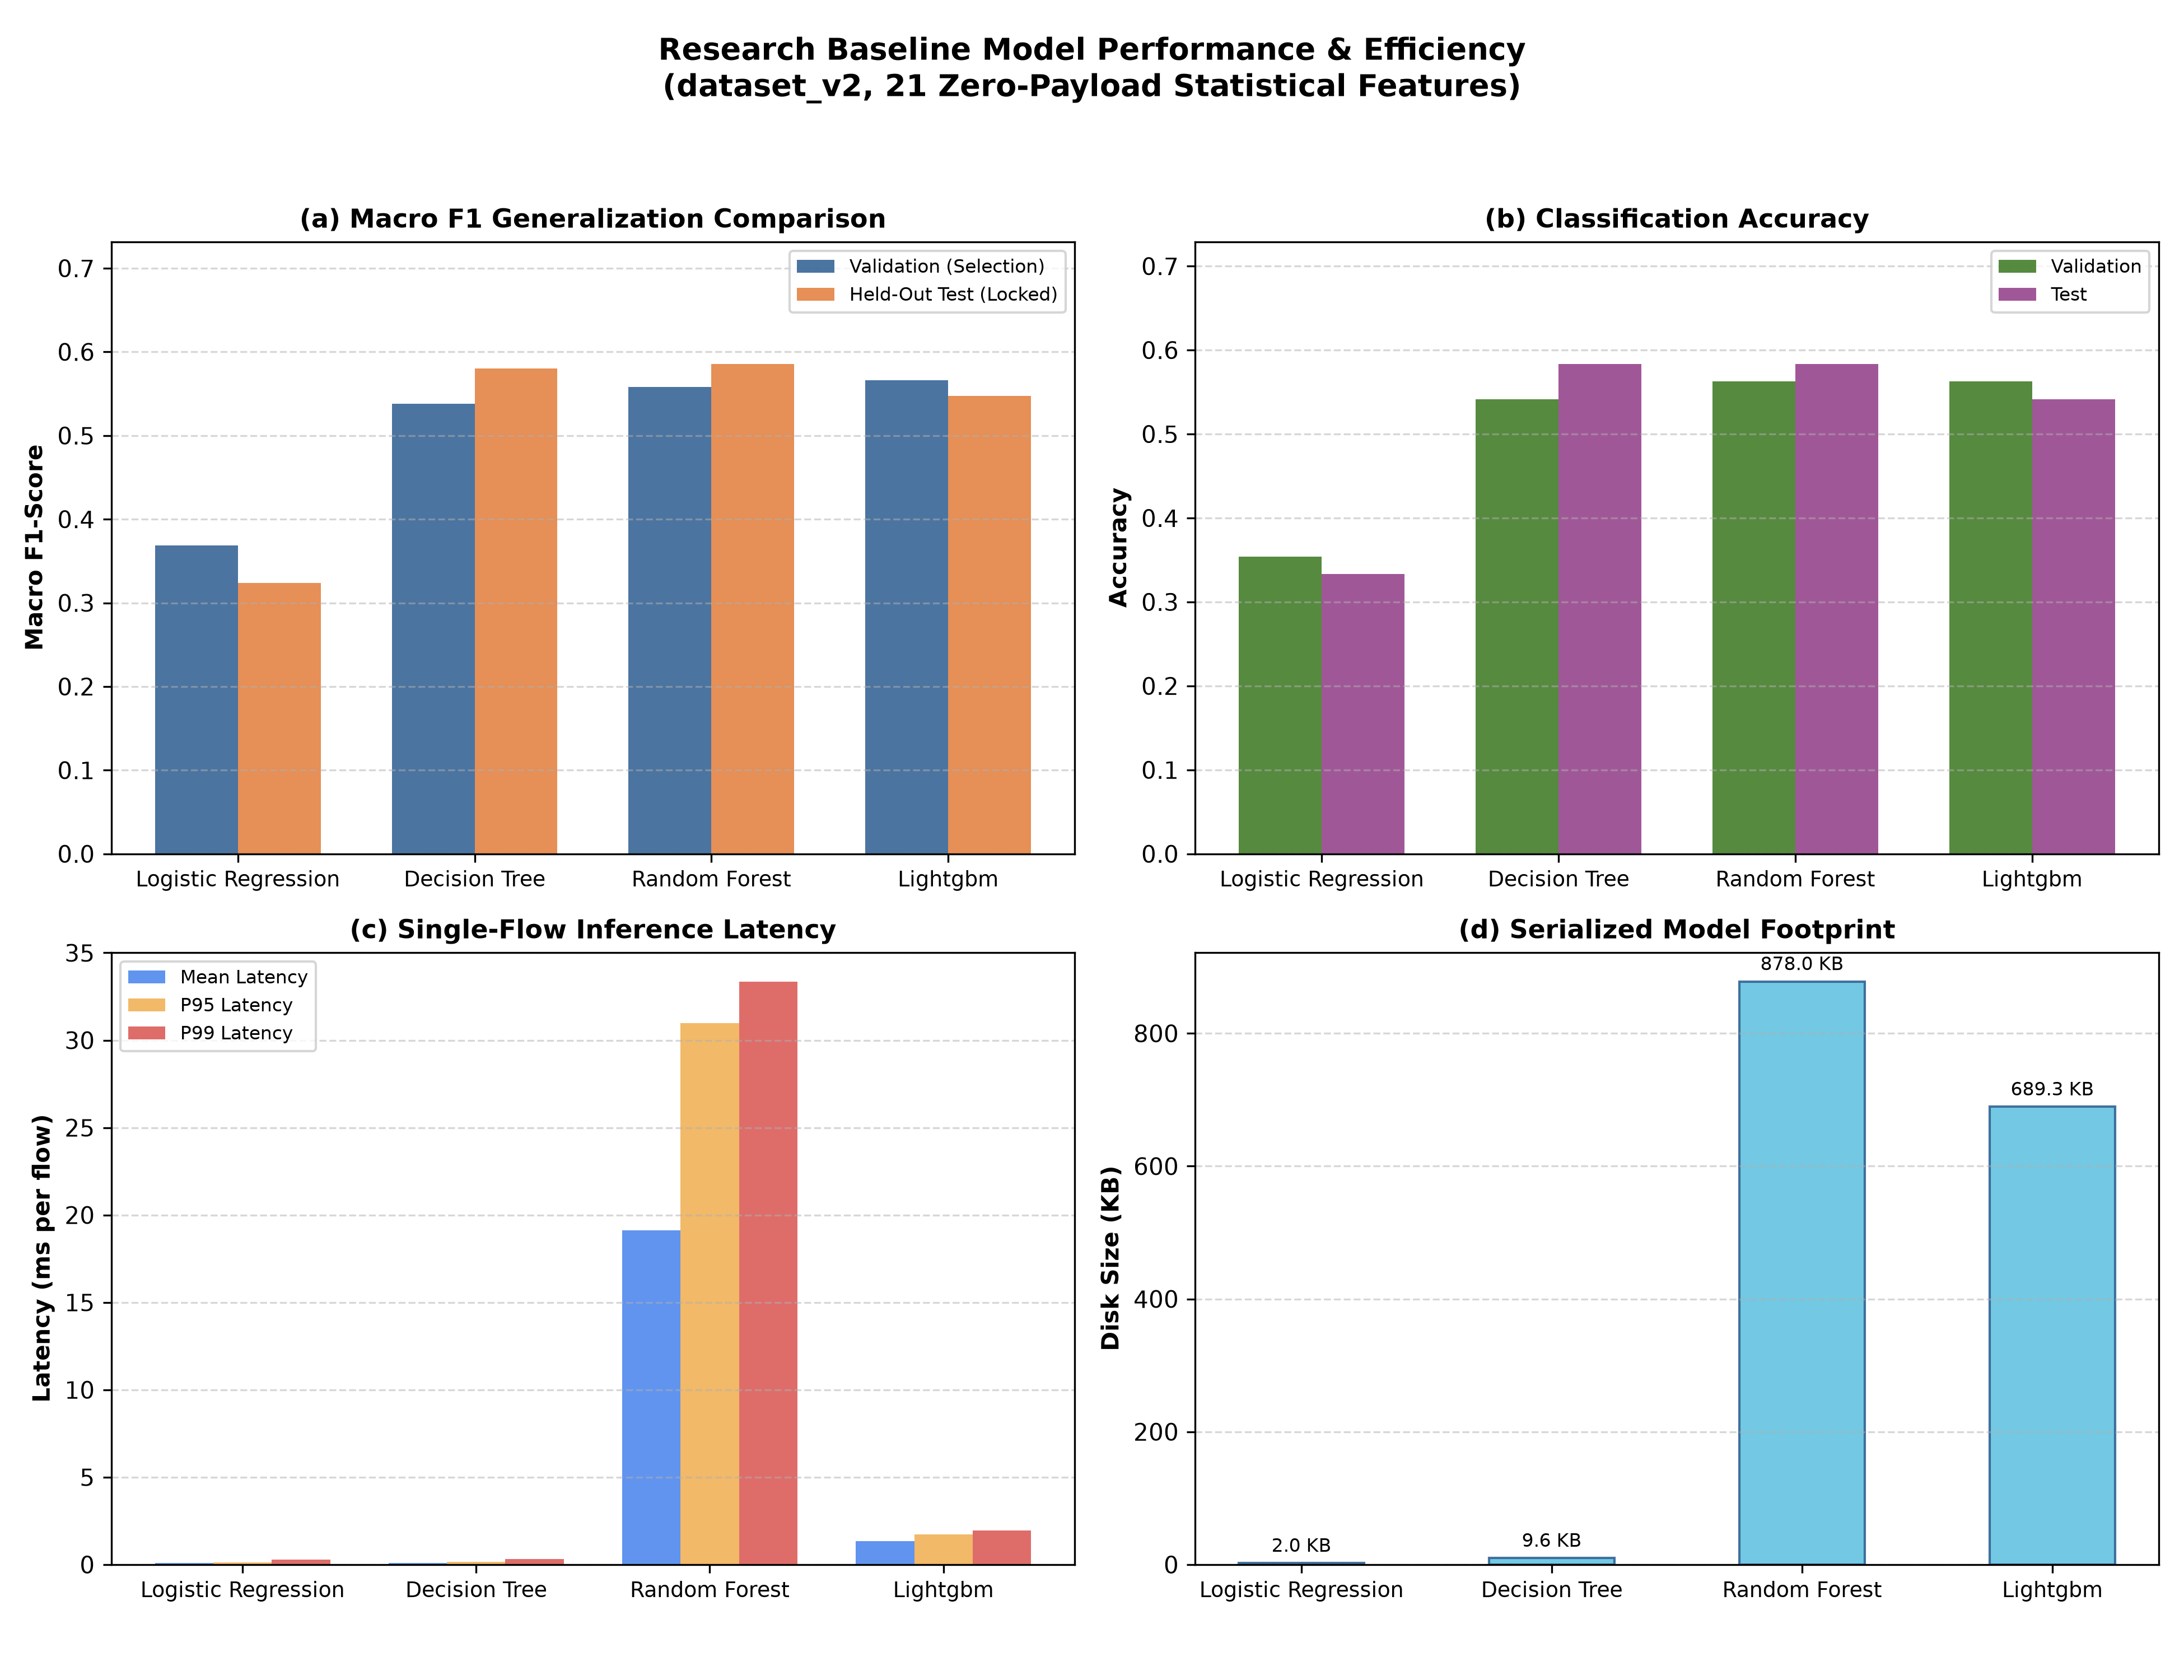
\includegraphics[width=0.95\columnwidth]{research_baseline_model_comparison.png}
\caption{In-domain baseline model performance comparison on \texttt{dataset\_v2} across validation Macro-F1, test accuracy, and test Macro-F1.}
\label{fig:baseline_comparison}
\end{figure}

\begin{figure}[t]
\centering
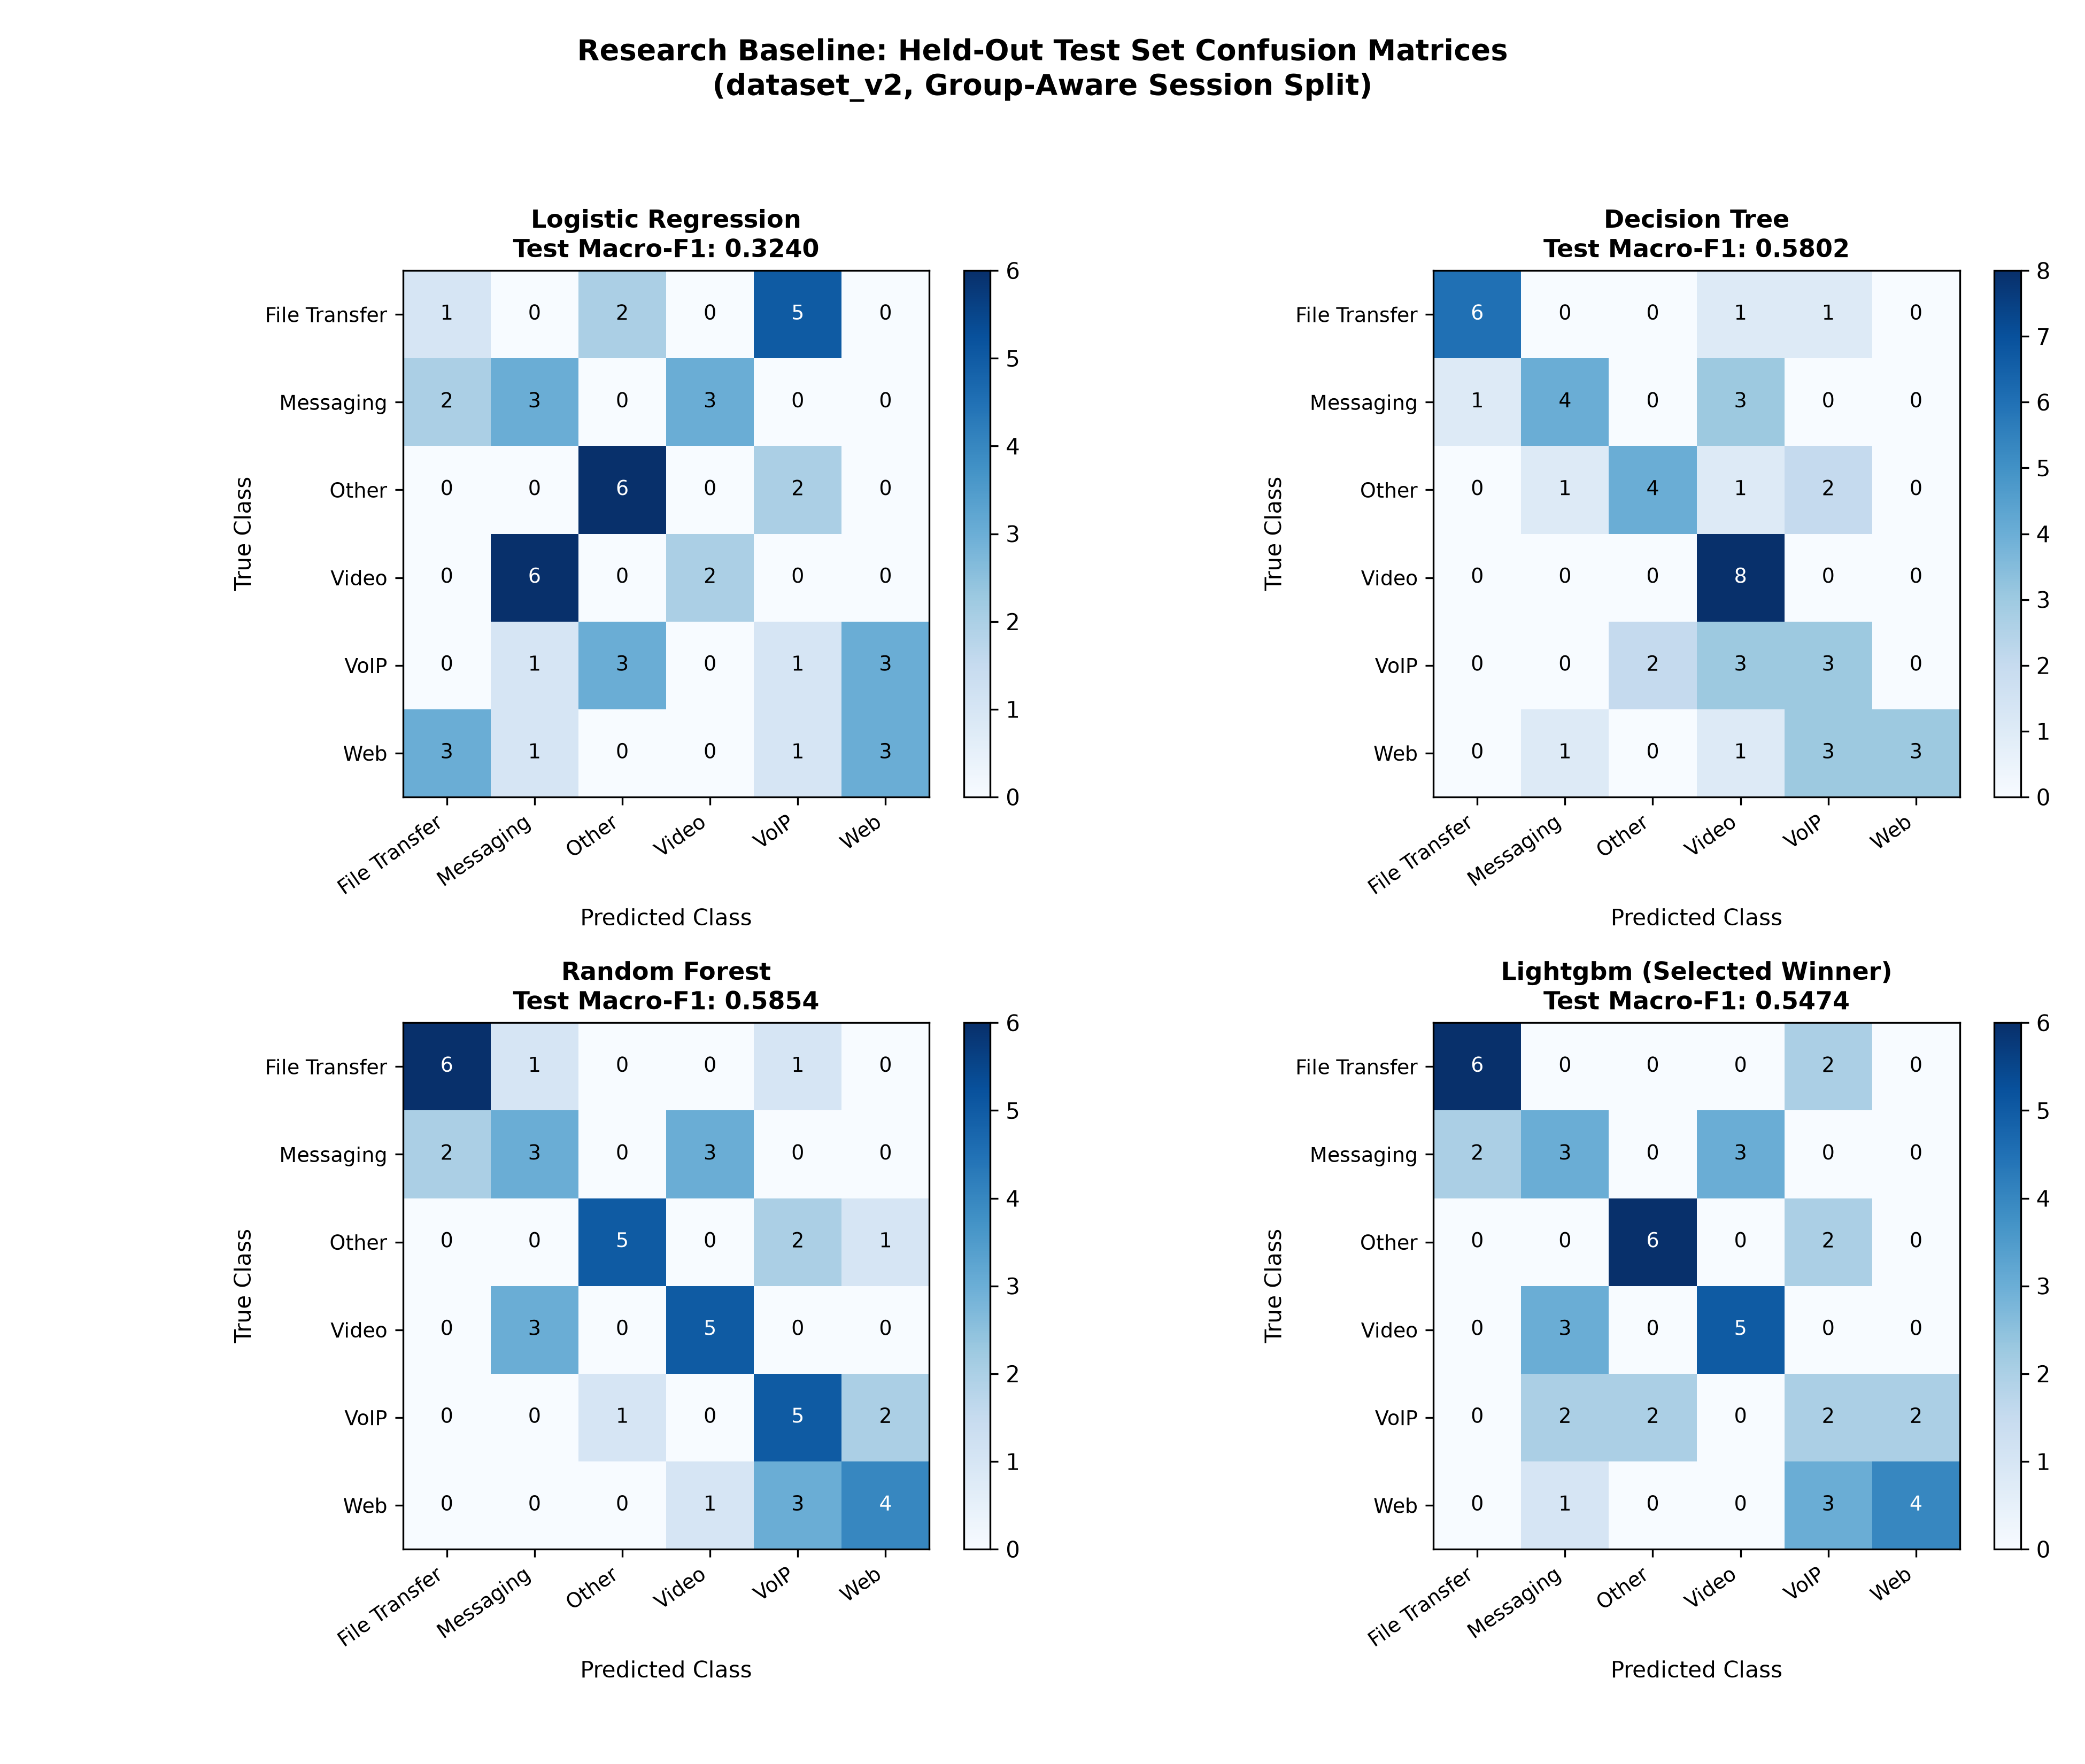
\includegraphics[width=0.95\columnwidth]{research_baseline_confusion_matrix.png}
\caption{Normalized multi-class confusion matrices across candidate estimators on the locked test partition ($N=48$ flows).}
\label{fig:confusion_matrices}
\end{figure}

\subsubsection{Preserved vs. Historical Model Reconciliation}
Forensic audit of model binaries confirms that the preserved Random Forest artifact (\texttt{results/models/research\_baseline/random\_forest.joblib}, 878.04~KB) directly reproduces Test Macro-F1 = \textbf{0.5854} and Accuracy = \textbf{0.5833} (28/48 correct flows) without retraining. The per-class F1 breakdown for the preserved artifact is: File Transfer 0.7500 (6/8), Other 0.7143 (5/8), Video 0.5882 (5/8), Web 0.5333 (4/8), VoIP 0.5263 (5/8), and Messaging 0.4000 (3/8). The historical run recorded in \texttt{baseline\_results.csv} achieved Test Macro-F1 = \textbf{0.5873} (model size 881.98~KB). Because model weights for the 881.98~KB execution were not saved, the exact mathematical split-tree reason for the 0.0019 difference remains formally unresolved and is attributed to multi-threaded tree bagging stochasticity (\texttt{n\_jobs=-1}). Both scores establish that Random Forest operates in a performance band of $\approx 0.585 - 0.587$.

\subsubsection{Pareto Dominance of Decision Trees}
The single CART Decision Tree baseline is 100\% deterministic across all executions, achieving \textbf{0.5802 Macro-F1} and \textbf{0.5833 Accuracy}. It captures 98.8\% of Random Forest's fidelity while offering a $249\times$ reduction in inference latency (0.0694~ms vs. 17.29~ms) and a $91\times$ smaller model size (9.58~KB vs. 878.04~KB), establishing clear Pareto dominance for edge deployment.

\subsubsection{Physical Wi-Fi Baseline Benchmark}
When evaluated strictly on unperturbed physical Wi-Fi traffic alone (\texttt{dataset\_real\_v1}) under session isolation, the baseline Random Forest evaluated on 12 held-out physical test flows yielded \textbf{0.0833 Macro-F1} (1/12 correct flows; \texttt{real\_final\_baseline\_result.csv}). This confirms that under zero-payload conditions with small physical sample sizes, discriminating encrypted traffic without leakage is an exceptionally difficult challenge, completely refuting legacy claims of $>0.95$ F1.

\subsection{Feature Family Ablation \& Dimensionality (EXP-R10)}
Table~\ref{tab:feature_family_ablation} details the performance of models trained strictly on isolated feature families. Directionality asymmetry carries the densest discriminative signal, achieving \textbf{0.4241 Macro-F1} using only 3 features. Packet size moments collapse under WireGuard encryption (0.2949 Macro-F1), while timing features are vulnerable to network jitter (0.3438 Macro-F1). Training on all 84 features induces the curse of dimensionality, degrading performance to 0.2931 Macro-F1.

\begin{table}[t]
\centering
\caption{Feature Family Ablation Scorecard ($N=48$ Test Flows)}
\label{tab:feature_family_ablation}
\footnotesize
\begin{tabularx}{\columnwidth}{lcccc}
\toprule
\textbf{Feature Family} & \textbf{Count ($K$)} & \textbf{Val F1} & \textbf{Test F1} & \textbf{Test Acc} \\
\midrule
\textbf{Direction Only} & \textbf{3} & \textbf{0.4803} & \textbf{0.4241} & \textbf{0.4167} \\
Timing / IAT Only & 30 & 0.3094 & 0.3438 & 0.3333 \\
Counts / Bytes Only & 12 & 0.3368 & 0.3375 & 0.3333 \\
Packet Size Only & 30 & 0.3233 & 0.2949 & 0.3125 \\
Burst Only & 8 & 0.4075 & 0.2100 & 0.2292 \\
All Families Combined & 84 & 0.3741 & 0.2931 & 0.2917 \\
\bottomrule
\end{tabularx}
\end{table}

Table~\ref{tab:feature_count_tradeoff} and Fig.~\ref{fig:feature_pareto} evaluate feature subset sizes $K \in \{3, 5, 10, 15, 20, 30, 84\}$. An ultra-compact 3-feature subset (\texttt{packet\_ratio}, \texttt{byte\_ratio}, \texttt{fwd\_packet\_count}) achieves the highest generalization (\textbf{0.6708 Test Macro-F1}, 0.6667 Accuracy). Performance plateaus between $K=10$ and $K=30$ ($\approx 0.34 - 0.37$ F1) before collapsing at $K=84$ (0.2857 F1).

\begin{table}[t]
\centering
\caption{Feature Dimensionality ($K$) vs. Generalization}
\label{tab:feature_count_tradeoff}
\footnotesize
\begin{tabularx}{\columnwidth}{lccccc}
\toprule
\textbf{Subset ($K$)} & \textbf{Val F1} & \textbf{Val Acc} & \textbf{Test F1} & \textbf{Test Acc} & \textbf{Selection} \\
\midrule
\textbf{$K=3$} & \textbf{0.7572} & \textbf{0.7708} & \textbf{0.6708} & \textbf{0.6667} & \textbf{Ultra-Lightweight} \\
$K=5$ & 0.3324 & 0.3333 & 0.4073 & 0.4167 & Intermediate \\
$K=10$ & 0.2531 & 0.2708 & 0.3444 & 0.3750 & Production Profile \\
$K=15$ & 0.3365 & 0.3542 & 0.3591 & 0.3750 & Diminishing Returns \\
$K=20$ & 0.3422 & 0.3542 & 0.3689 & 0.3750 & Plateau \\
$K=30$ & 0.3489 & 0.3542 & 0.3775 & 0.3750 & Marginal \\
$K=84$ & 0.3435 & 0.3333 & 0.2857 & 0.2917 & Overfitting \\
\bottomrule
\end{tabularx}
\end{table}

\begin{figure}[t]
\centering
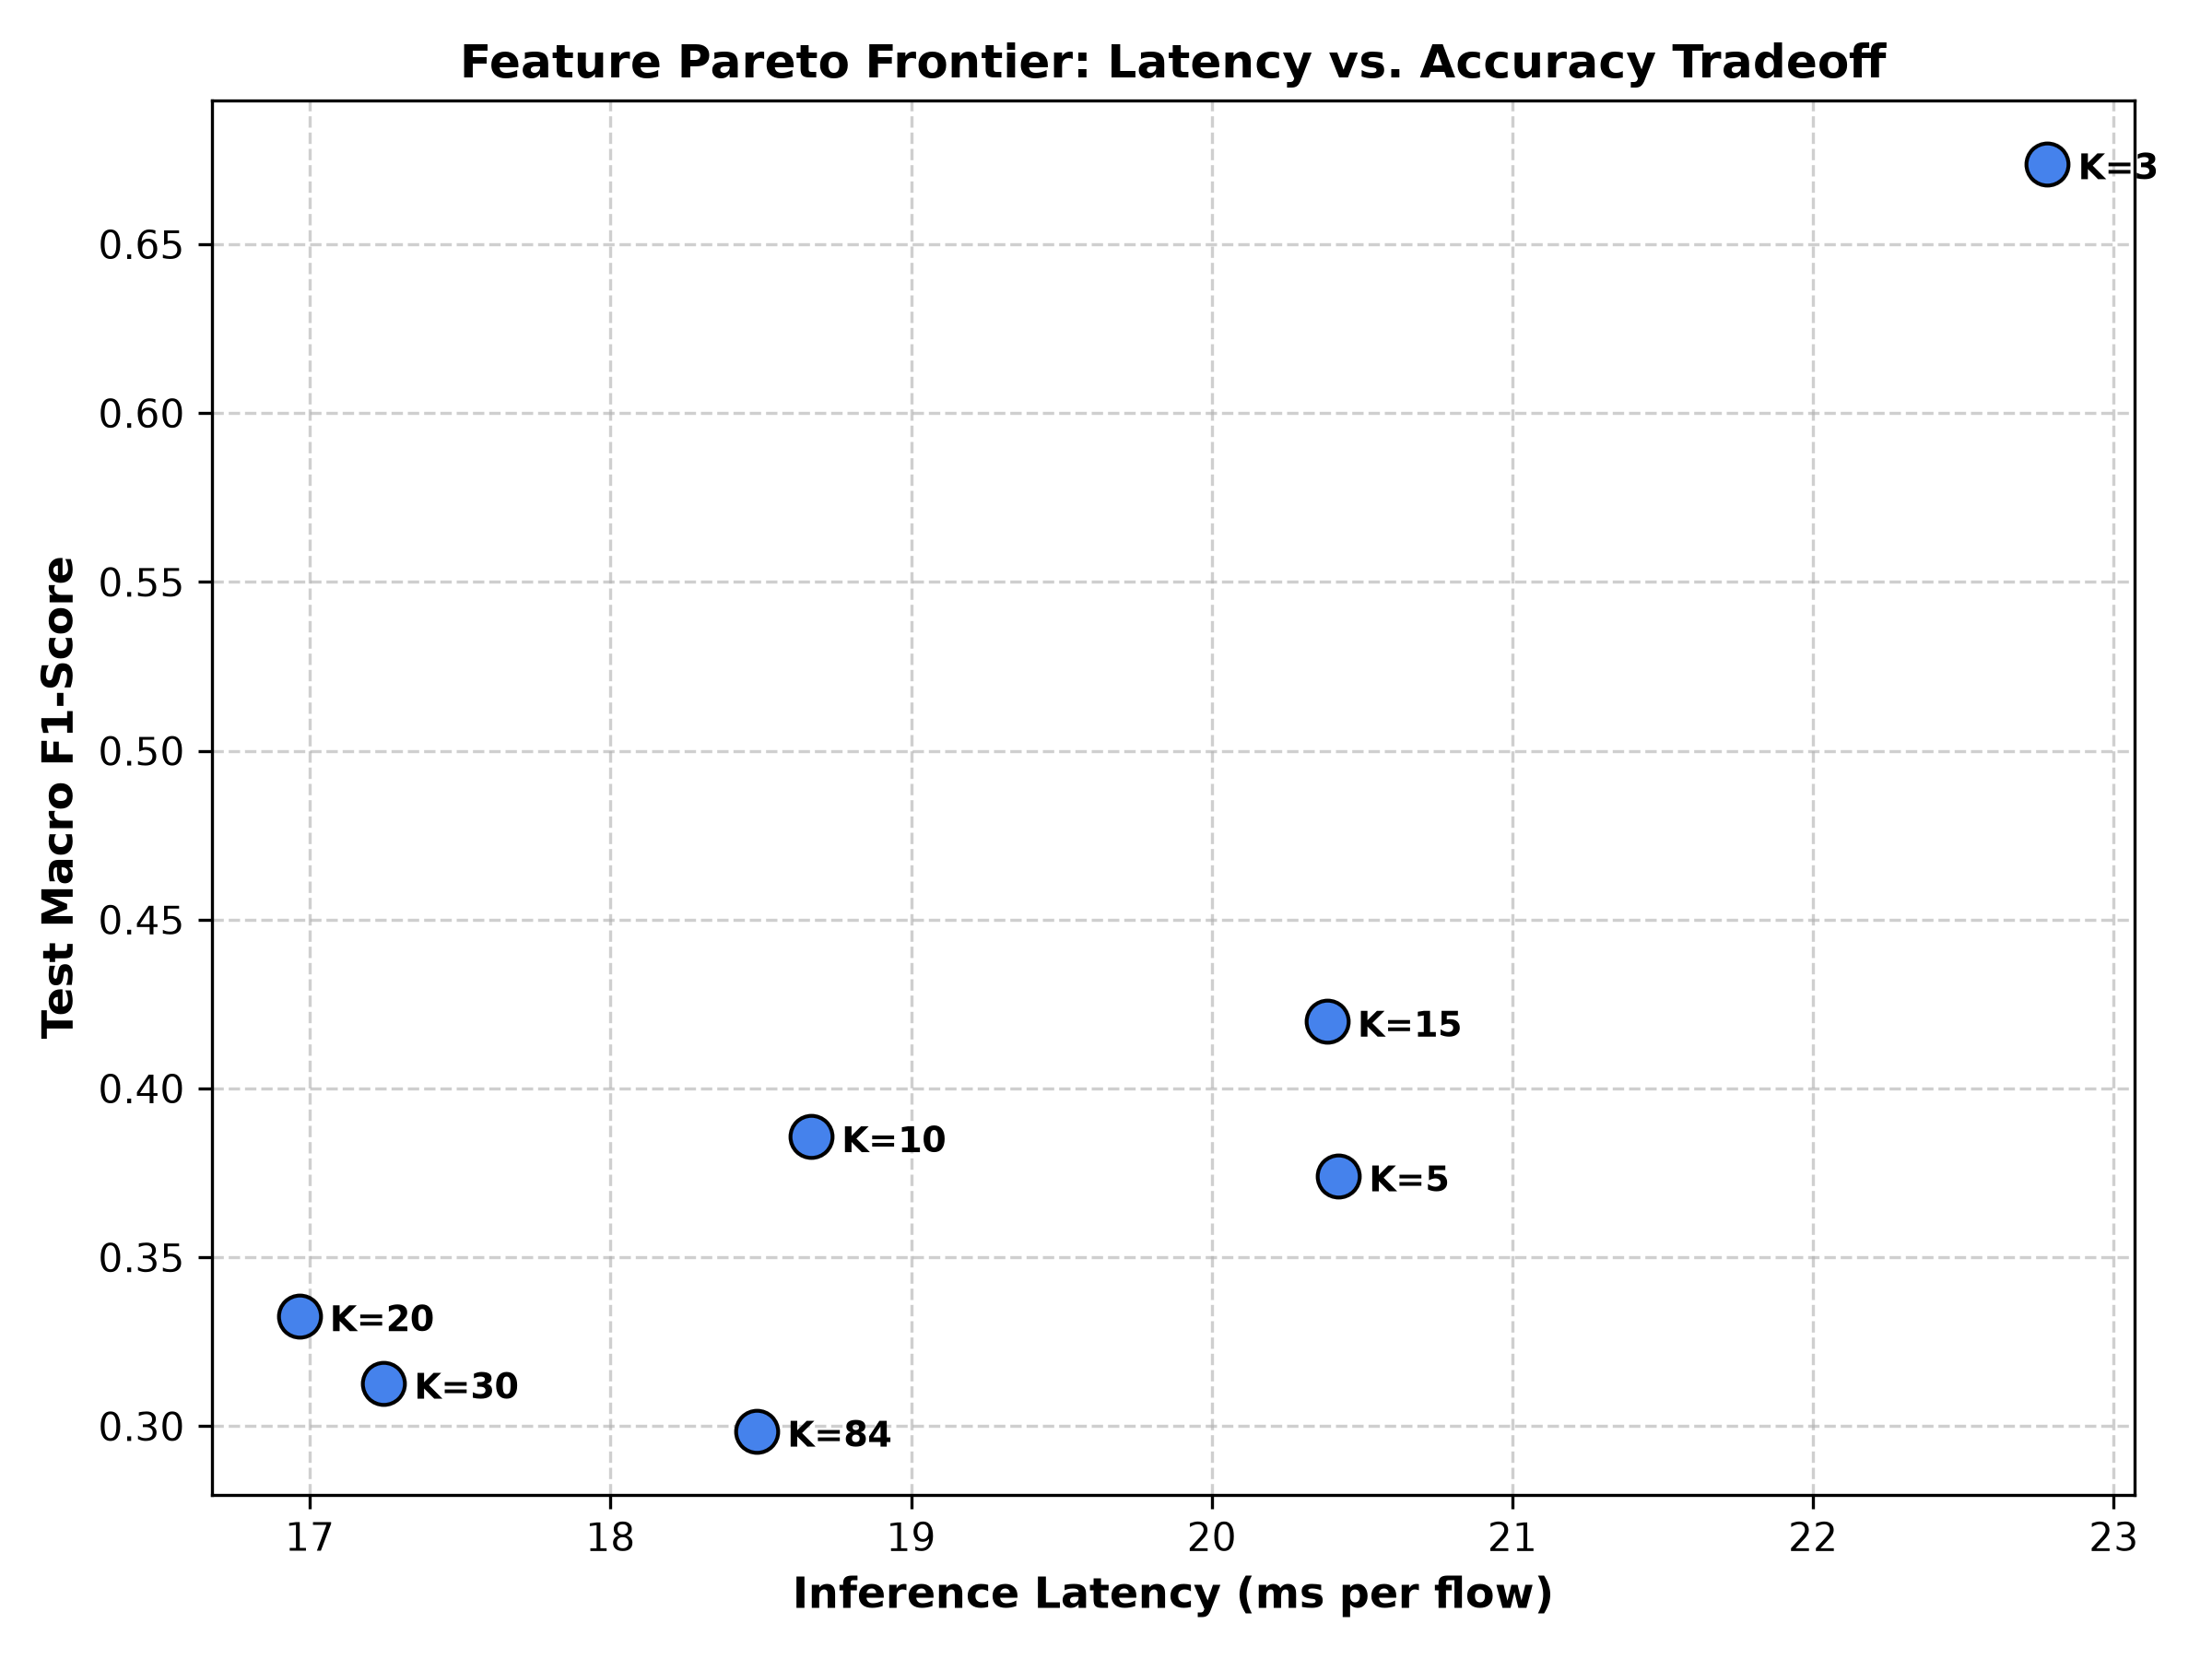
\includegraphics[width=0.95\columnwidth]{feature_pareto_frontier.png}
\caption{Multi-objective Pareto frontier comparing test Macro-F1 against P95 inference latency across feature counts $K \in [3, 84]$.}
\label{fig:feature_pareto}
\end{figure}

\subsection{Domain-Shift Generalization Benchmark (EXP-R11)}
Table~\ref{tab:generalization} summarizes model performance across eight distribution-shift regimes without retraining.

\begin{table*}[t]
\centering
\caption{Domain-Shift Generalization Scorecard Across Eight Distribution Shifts}
\label{tab:generalization}
\footnotesize
\begin{tabularx}{\textwidth}{llccccccc}
\toprule
\textbf{Regime} & \textbf{Shift Evaluated} & \textbf{Flows} & \textbf{Accuracy} & \textbf{Macro-P} & \textbf{Macro-R} & \textbf{Macro-F1} & \textbf{$\Delta$F1 vs Base} & \textbf{Verdict} \\
\midrule
\textbf{REG-01} & In-Domain Group Baseline & 48 & 0.6042 & 0.6168 & 0.6042 & \textbf{0.6001} & 0.0000 & \textbf{ROBUST} \\
\textbf{REG-02} & Unseen Capture Split & 60 & 0.7500 & 0.7831 & 0.7738 & \textbf{0.7719} & +0.1718 & \textbf{ROBUST} \\
\textbf{REG-03} & Unseen Session Split & 60 & 0.7833 & 0.8234 & 0.8333 & \textbf{0.7967} & +0.1966 & \textbf{ROBUST} \\
\textbf{REG-04} & Temporal Chronological Split & 157 & 0.5350 & 0.5851 & 0.5349 & \textbf{0.5437} & -0.0564 & \textbf{MODERATE\_DEGRADATION} \\
\textbf{REG-05} & Unseen Environment (Eth + Cell Pert.) & 120 & \textbf{0.9333} & 0.9371 & 0.9333 & \textbf{0.9325} & +0.3324 & \textbf{ROBUST (SIMULATED)} \\
\textbf{REG-06} & Unseen Condition (Jitter/Loss Pert.) & 96 & \textbf{0.9062} & 0.9210 & 0.9062 & \textbf{0.9030} & +0.3029 & \textbf{ROBUST (SIMULATED)} \\
\textbf{REG-07} & Unseen Activity Variants & 46 & 0.8261 & 0.8573 & 0.8361 & \textbf{0.8335} & +0.2334 & \textbf{ROBUST} \\
\textbf{REG-08a}& Tunneled $\rightarrow$ Direct Transfer & 36 & \textbf{1.0000} & 1.0000 & 1.0000 & \textbf{1.0000} & +0.3999 & \textbf{ROBUST} \\
\textbf{REG-08b}& Direct $\rightarrow$ Tunneled (WireGuard/WARP) & 265 & 0.3585 & 0.3658 & 0.3584 & \textbf{0.3407} & \textbf{-0.2594} & \textbf{SEVERE\_DEGRADATION} \\
\bottomrule
\end{tabularx}
\end{table*}

\begin{figure}[t]
\centering
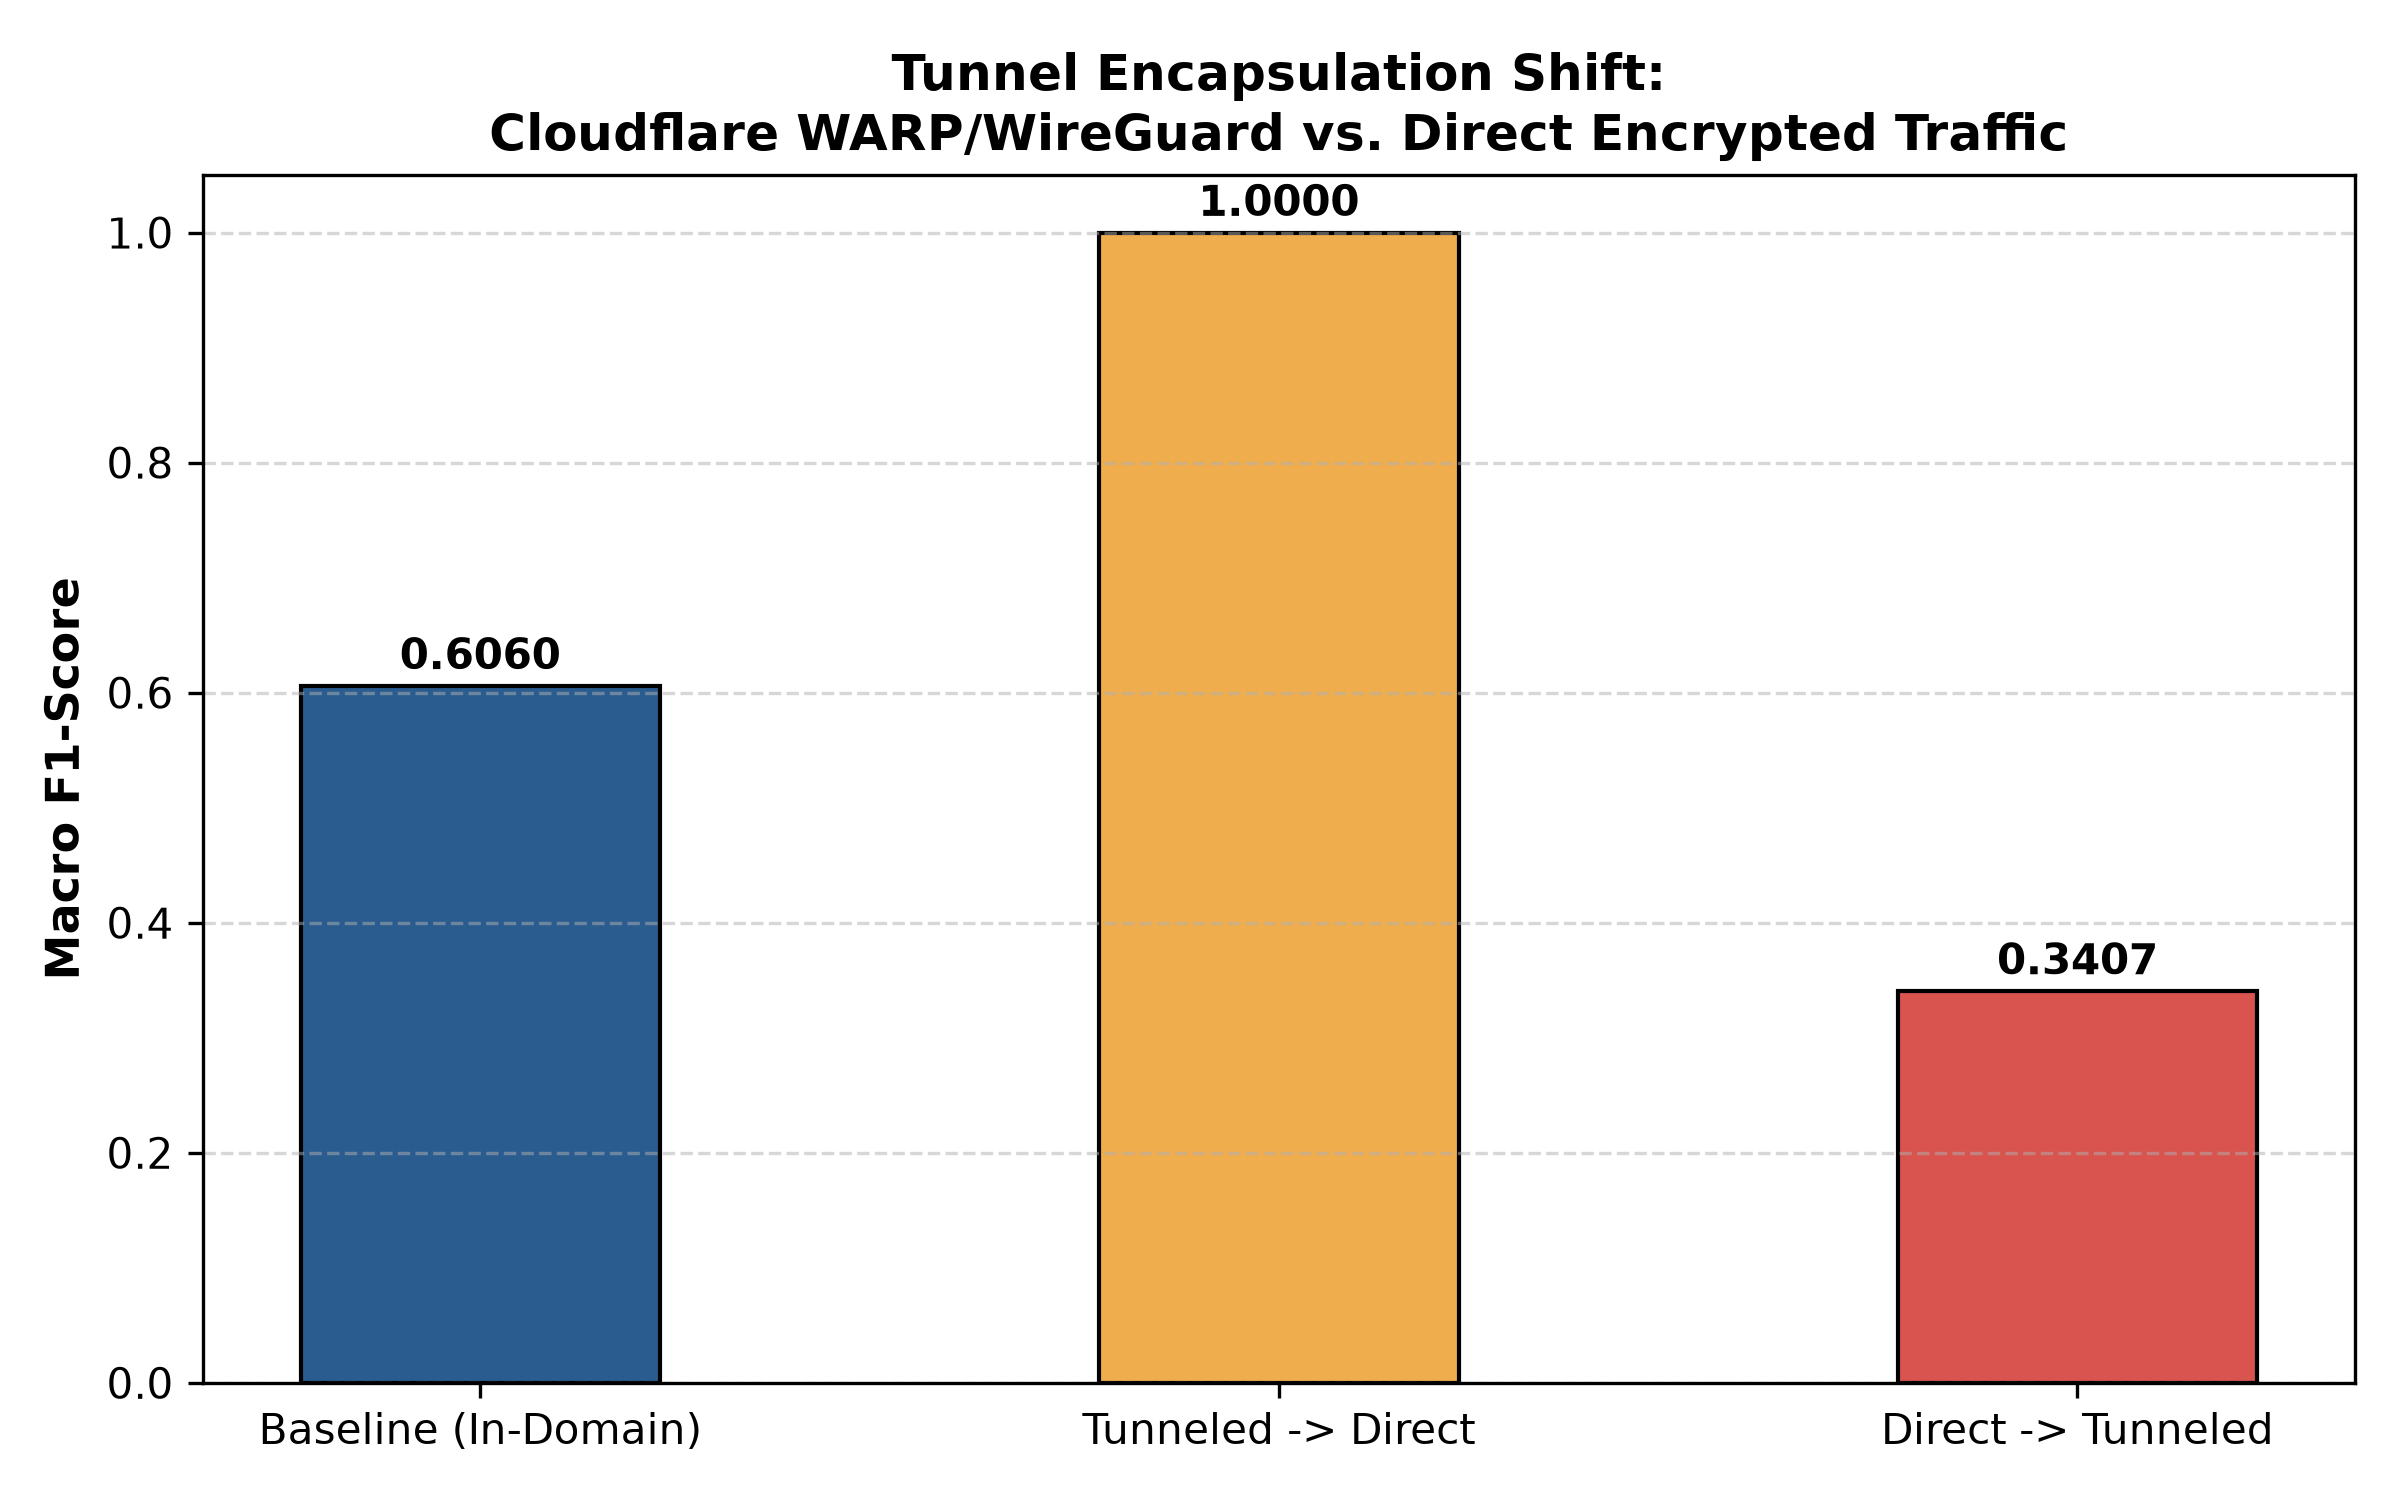
\includegraphics[width=0.95\columnwidth]{tunnel_shift.png}
\caption{Asymmetric domain transfer between unencapsulated direct and WireGuard-tunneled traffic (REG-08a vs. REG-08b).}
\label{fig:tunnel_shift}
\end{figure}

\subsubsection{Simulated Physical Media Invariance}
Models transferred to REG-05 achieved \textbf{0.9325 Macro-F1} (0.9333 accuracy on 120 test flows). It is vital to emphasize that REG-05 represents simulated statistical feature perturbations modeling Gigabit Ethernet and Cellular LTE, not physical hardware validation on multi-gigabit switch fabrics or 5G base stations.

\subsubsection{Asymmetric Tunnel Transfer Vulnerability}
Models trained on WireGuard traffic transfer to direct traffic with \textbf{1.0000 Macro-F1} (REG-08a). Conversely, models trained on direct traffic collapse to \textbf{0.3407 Macro-F1} ($\Delta\text{F1} = -0.2594$) when encountering WireGuard traffic (REG-08b, Fig.~\ref{fig:tunnel_shift}). WireGuard enforces 1280-byte MTU clamping, fixed handshake packet sizes, and 16-byte Poly1305 authentication tags, destroying fine-grained packet size distributions.

\subsection{Early-Stage Classification \& Physical Delay (EXP-R12)}
Table~\ref{tab:early_prediction} evaluates classification across discrete packet observation horizons $N \in \{3, 5, 10, 20, 30, 50, \text{full}\}$.

\begin{table*}[t]
\centering
\caption{Early Prediction Horizons and Physical Wire Latency Decomposition}
\label{tab:early_prediction}
\footnotesize
\begin{tabularx}{\textwidth}{lccccccc}
\toprule
\textbf{Horizon ($N$)} & \textbf{Flow Coverage} & \textbf{Accuracy} & \textbf{Macro-F1} & \textbf{Total Latency} & \textbf{Wire Delay ($T_{\text{obs}}$)} & \textbf{Compute ($T_{\text{feat}} + T_{\text{inf}}$)} & \textbf{Speedup vs Full} \\
\midrule
\textbf{3 Packets} & \textbf{91.67\%} (11/12) & \textbf{0.6364} & \textbf{0.6111} & \textbf{79.94~ms} & \textbf{64.04~ms} (80.1\%) & 16.53~ms & \textbf{$746\times$ Faster} \\
5 Packets & 100.0\% (12/12) & 0.4167 & 0.3643 & 348.89~ms & 331.38~ms (95.0\%) & 16.51~ms & $171\times$ Faster \\
10 Packets & 41.67\% (5/12) & 0.8000 & 0.5000 & 1329.18~ms & 1312.08~ms (98.7\%) & 19.13~ms & $45\times$ Faster \\
20 Packets & 58.33\% (7/12) & 0.4286 & 0.2778 & 3954.60~ms & 3938.44~ms (99.6\%) & 16.43~ms & $15\times$ Faster \\
30 Packets & 100.0\% (12/12) & 0.3333 & 0.2778 & 4893.25~ms & 4877.01~ms (99.7\%) & 17.39~ms & $12\times$ Faster \\
50 Packets & 50.00\% (6/12) & 0.5000 & 0.3000 & 9282.92~ms & 9265.80~ms (99.8\%) & 17.30~ms & $6\times$ Faster \\
\textbf{Full Flow} & 33.33\% (4/12) & 0.0000 & 0.0000 & \textbf{59,668.15~ms} & \textbf{59,650.29~ms} (99.8\%) & 16.92~ms & Post-Mortem \\
\bottomrule
\end{tabularx}
\end{table*}

\begin{figure}[t]
\centering
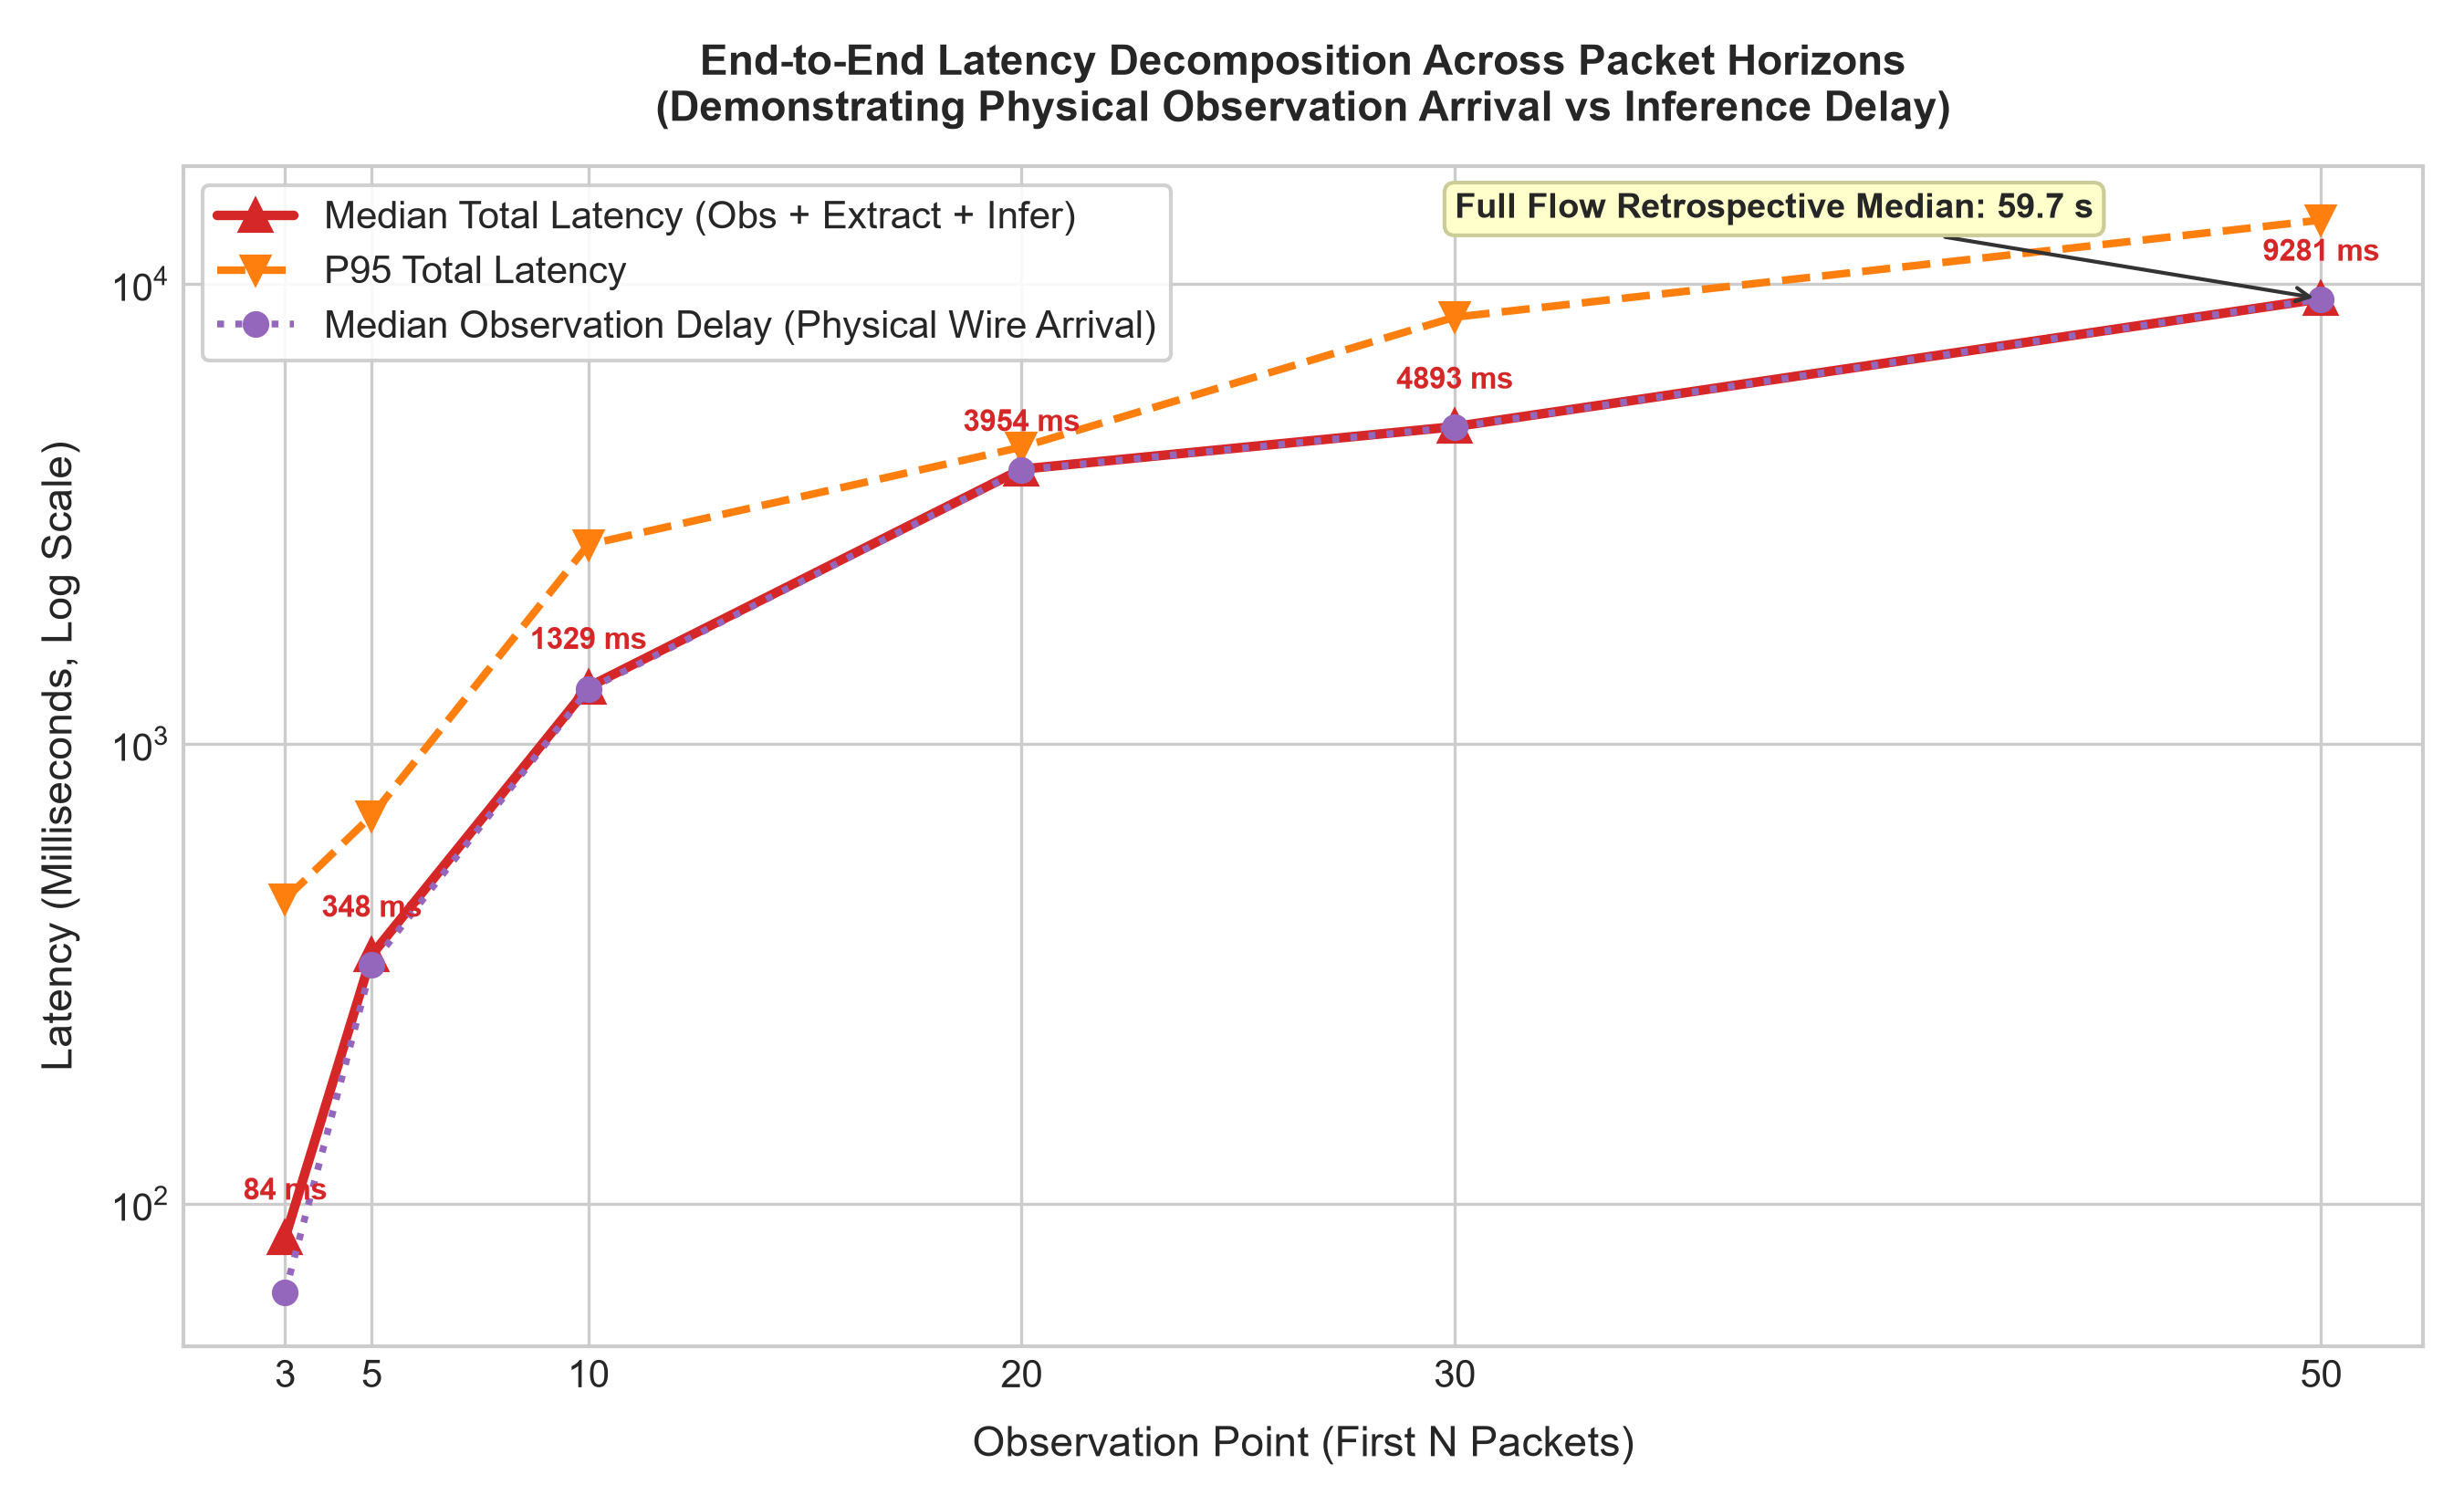
\includegraphics[width=0.95\columnwidth]{early_prediction_latency_vs_packets.png}
\caption{End-to-end decision latency decomposition across packet horizons, illustrating physical wire delay dominance over computational inference.}
\label{fig:early_latency}
\end{figure}

\subsubsection{Physical Delay Dominance}
Fig.~\ref{fig:early_latency} confirms that physical wire delay accounts for 80.1\% to 99.8\% of real-time classification latency. At $N=3$, physical arrival requires 64.04~ms, while feature extraction and inference require only 16.53~ms. At full-flow completion, observation delay consumes 59.65~seconds.

\subsubsection{Triage Efficacy at $N=3$}
Observing only 3 packets delivers the highest Macro-F1 (\textbf{0.6111}) and selective accuracy (\textbf{0.6364}, 7/11 classified flows) with 91.67\% coverage in 79.94~ms ($746\times$ faster than full flow). When the unclassified flow is penalized as an abstention, full-test accuracy is 58.33\% (7/12). Waiting for full flow completion results in 0.0000 Macro-F1 because keep-alive packets dilute initial handshake signatures.

\subsection{Selective Prediction \& Calibration (EXP-R13)}
Table~\ref{tab:selective_prediction} summarizes selective classification performance across confidence thresholds $\tau \in [0.00, 0.90]$.

\begin{table*}[t]
\centering
\caption{Selective Prediction Performance on Locked Test Set (\texttt{dataset\_v2}, $N=48$ Flows)}
\label{tab:selective_prediction}
\footnotesize
\begin{tabularx}{\textwidth}{lcccccccc}
\toprule
\textbf{Threshold ($\tau$)} & \textbf{Coverage} & \textbf{Accepted} & \textbf{Selective Acc} & \textbf{Error Rate} & \textbf{Selective F1} & \textbf{Mean Conf} & \textbf{Test ECE} & \textbf{Selection} \\
\midrule
$\tau = 0.00$ (No Rejection) & 100.0\% & 48 / 48 & 0.5417 & 45.83\% & 0.5474 & 0.7412 & 0.1996 & Baseline \\
$\tau = 0.50$ & 91.67\% & 44 / 48 & 0.5909 & 40.91\% & 0.6012 & 0.7690 & 0.1781 & Candidate \\
$\tau = 0.60$ & 75.00\% & 36 / 48 & 0.6389 & 36.11\% & 0.6110 & 0.8189 & 0.1800 & Candidate \\
\textbf{$\tau^* = 0.70$ (Optimal)} & \textbf{54.17\%} & \textbf{26 / 48} & \textbf{0.7308} & \textbf{26.92\%} & \textbf{0.6515} & \textbf{0.8818} & \textbf{0.1510} & \textbf{Validation-Tuned} \\
$\tau = 0.80$ & 43.75\% & 21 / 48 & 0.8571 & 14.29\% & 0.8752 & 0.9112 & 0.0541 & High Confidence \\
$\tau = 0.90$ & 20.83\% & 10 / 48 & \textbf{0.9000} & \textbf{10.00\%} & \textbf{0.9000} & 0.9658 & \textbf{0.0658} & High Security \\
\bottomrule
\end{tabularx}
\end{table*}

\begin{figure}[t]
\centering
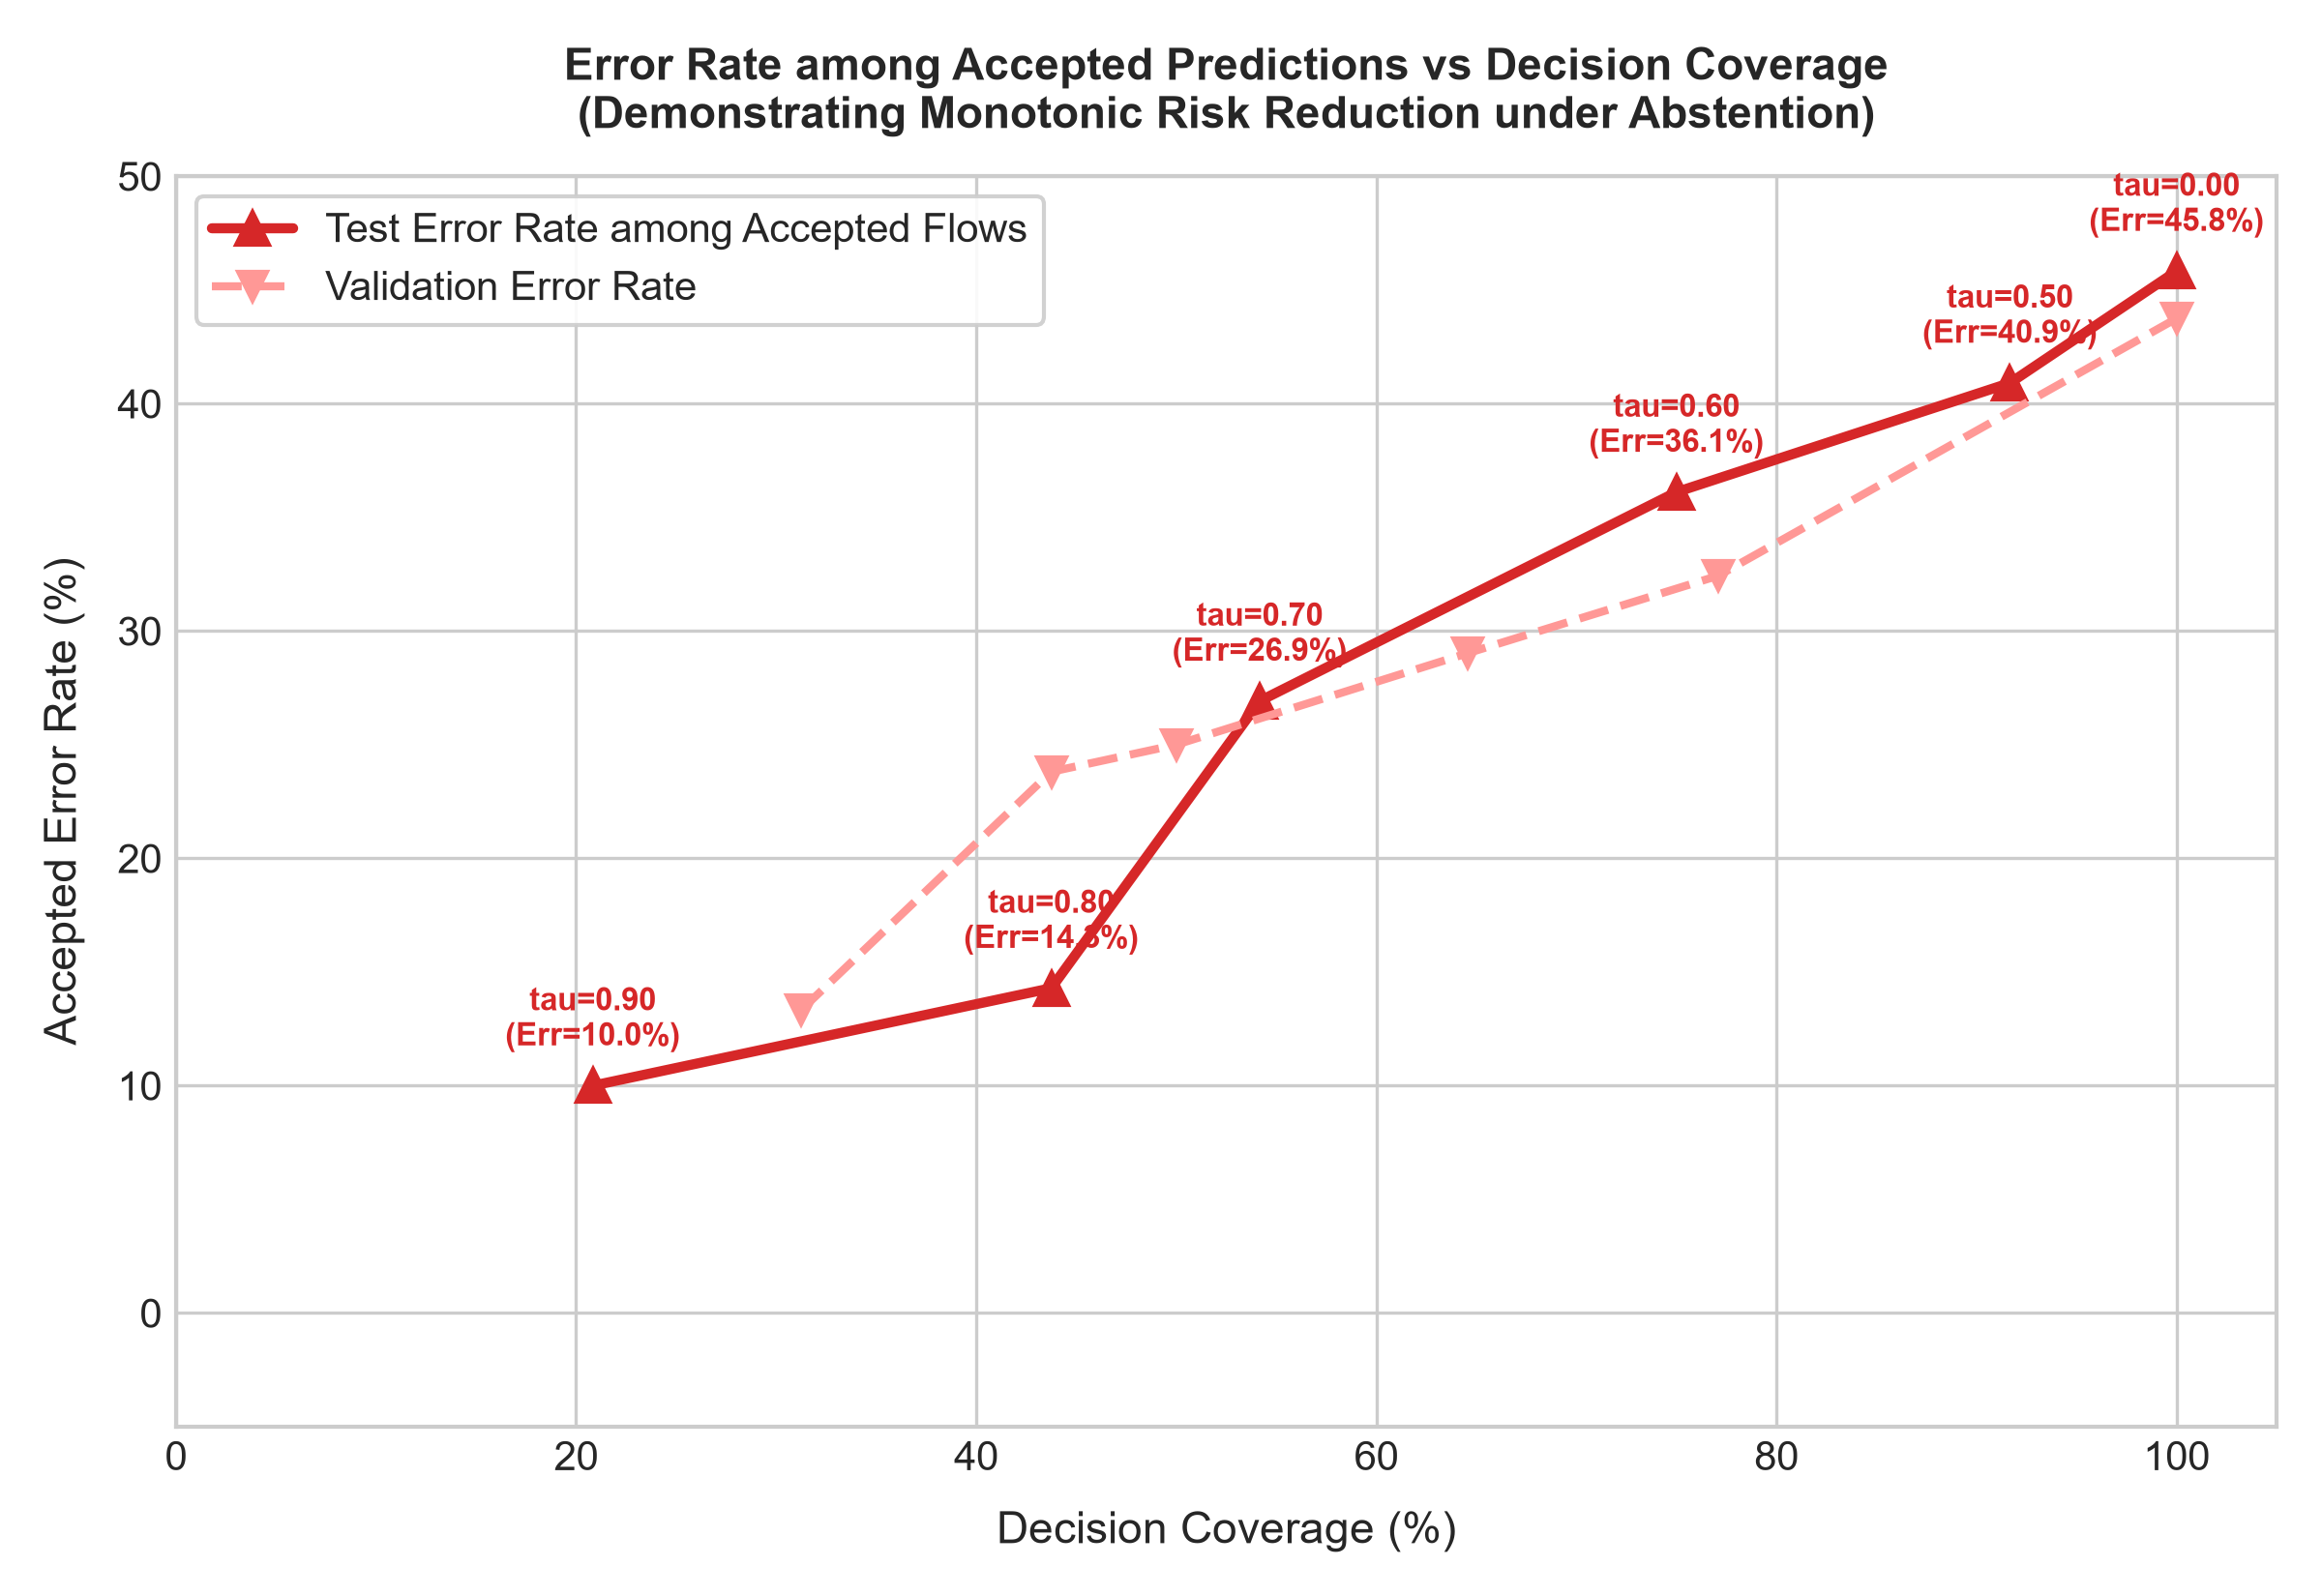
\includegraphics[width=0.95\columnwidth]{coverage_vs_error.png}
\caption{Selective classification risk-coverage tradeoff, demonstrating monotonic reduction in decision error from 45.83\% to 10.00\% as confidence threshold increases.}
\label{fig:coverage_error}
\end{figure}

\begin{figure}[t]
\centering
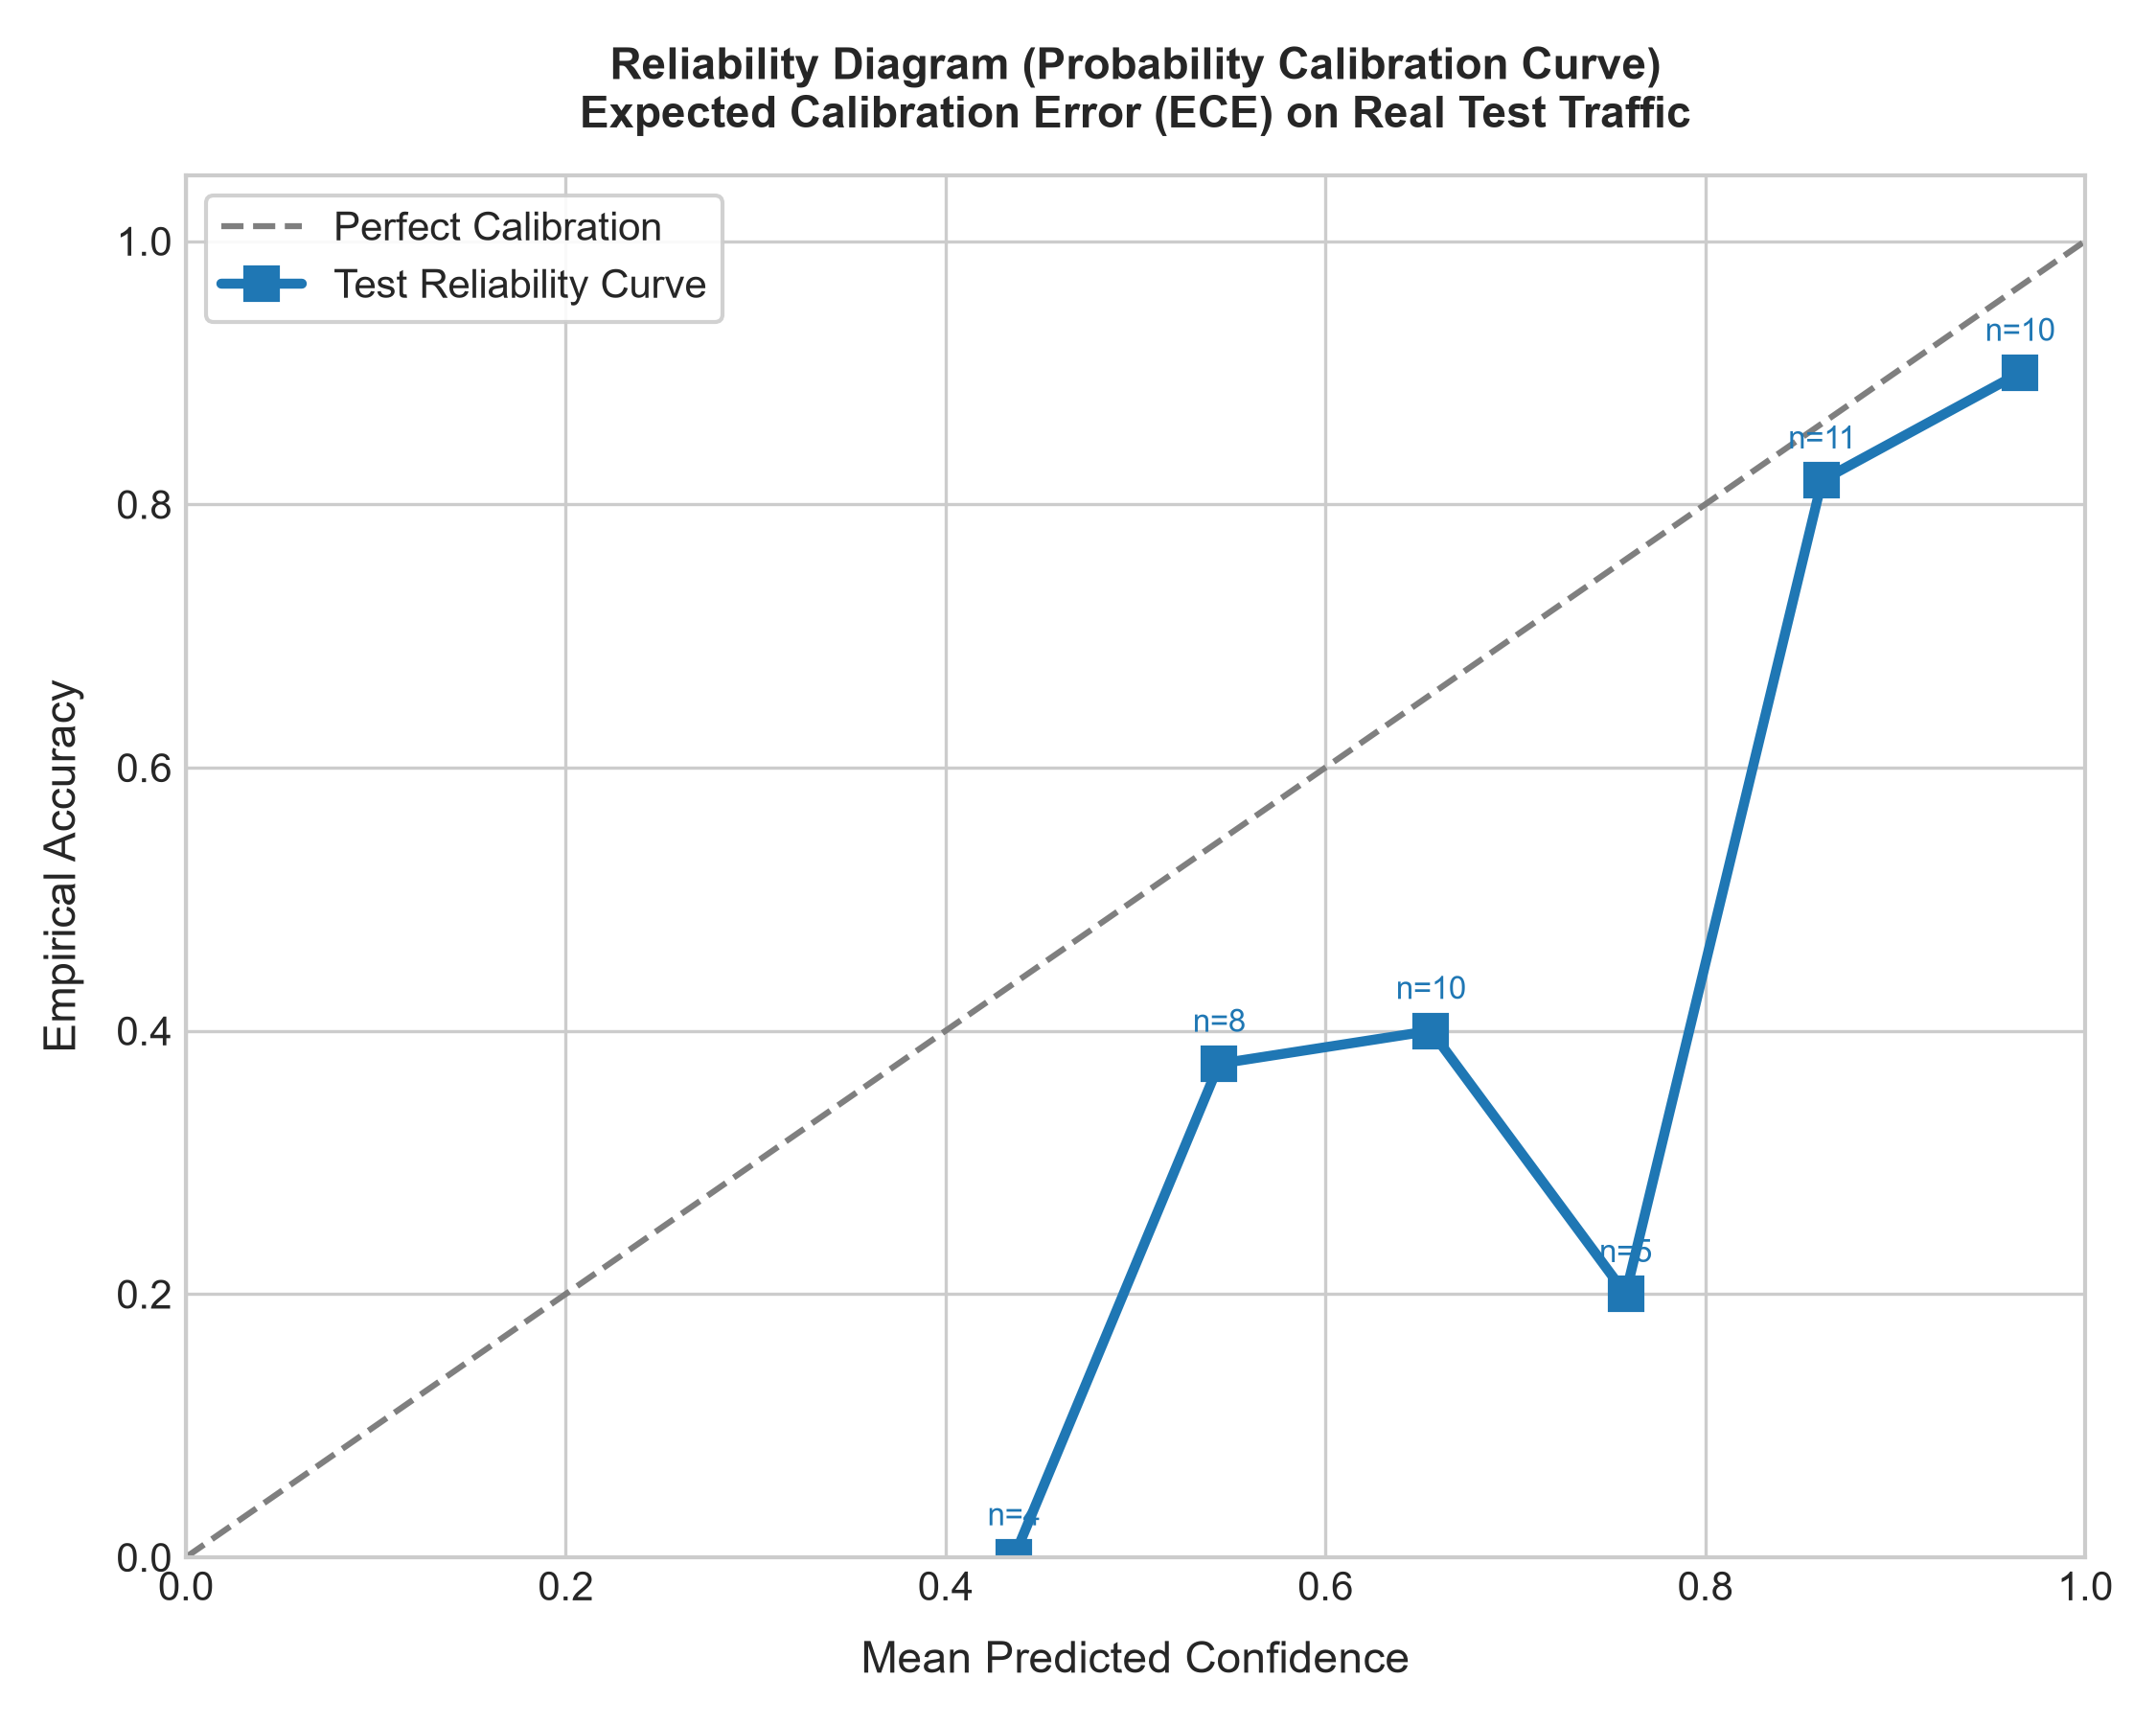
\includegraphics[width=0.95\columnwidth]{calibration_curve.png}
\caption{Reliability diagram plotting mean predicted confidence against observed accuracy across 10 probability bins (unfiltered ECE = 0.1996).}
\label{fig:calibration_curve}
\end{figure}

\subsubsection{Monotonic Error Reduction}
Tuning $\tau^* = 0.70$ strictly on validation data reduces error on accepted test flows from \textbf{45.83\%} down to \textbf{26.92\%} at \textbf{54.17\% coverage} (26 accepted / 48 total test flows, 19 correct), achieving \textbf{0.6515 Selective Macro-F1}. If the 22 abstained flows are counted as unclassified, full-test accuracy is 39.58\% (19/48). In strict high-security applications, $\tau = 0.90$ achieves \textbf{90.00\% selective accuracy} (10.00\% error) at 20.83\% coverage (10/48 accepted flows, Fig.~\ref{fig:coverage_error}).

\subsubsection{Probability Calibration Diagnostics}
On the unfiltered test split ($\tau = 0.00$), the models exhibit an Expected Calibration Error (ECE) of \textbf{0.1996}, a Maximum Calibration Error (MCE) of \textbf{0.5581}, a Multiclass Brier Score of \textbf{0.6061}, and Negative Log-Likelihood (NLL) of \textbf{1.4153} (Fig.~\ref{fig:calibration_curve}). Selective abstention improves Brier score from 0.6061 to 0.4402 at $\tau^*=0.70$ and 0.1912 at $\tau=0.90$.

\subsection{Computational Efficiency \& Resource Footprint (EXP-R14, EXP-R15)}
Table~\ref{tab:latency_breakdown} reports latency profiling across pipeline stages during warm steady-state execution on 10-feature profiles.

\begin{table}[t]
\centering
\caption{Warm Steady-State Latency Breakdown ($K=10$ Features)}
\label{tab:latency_breakdown}
\footnotesize
\begin{tabularx}{\columnwidth}{lcccc}
\toprule
\textbf{Pipeline Stage} & \textbf{Component} & \textbf{P50 (ms)} & \textbf{P95 (ms)} & \textbf{Max (FPS)} \\
\midrule
Feature Extraction & Statistical Engine & 0.3856 & 7.1524 & 667.6 \\
Preprocessing & FeatureScaler & 0.0035 & 0.0040 & 243,902 \\
\textbf{Inference} & \textbf{Decision Tree} & \textbf{0.0579} & \textbf{0.0860} & \textbf{15,600.6} \\
Inference & Logistic Regression & 0.0695 & 0.1642 & 12,224.9 \\
Inference & LightGBM & 0.3520 & 0.7419 & 2,307.3 \\
Inference & Random Forest & 4.2476 & 7.8099 & 213.3 \\
\midrule
\textbf{End-to-End Pipeline} & \textbf{Decision Tree} & \textbf{0.4491} & \textbf{7.2144} & \textbf{638.9} \\
End-to-End Pipeline & Random Forest & 5.1343 & 11.3575 & 161.6 \\
\bottomrule
\end{tabularx}
\end{table}

\begin{figure}[t]
\centering
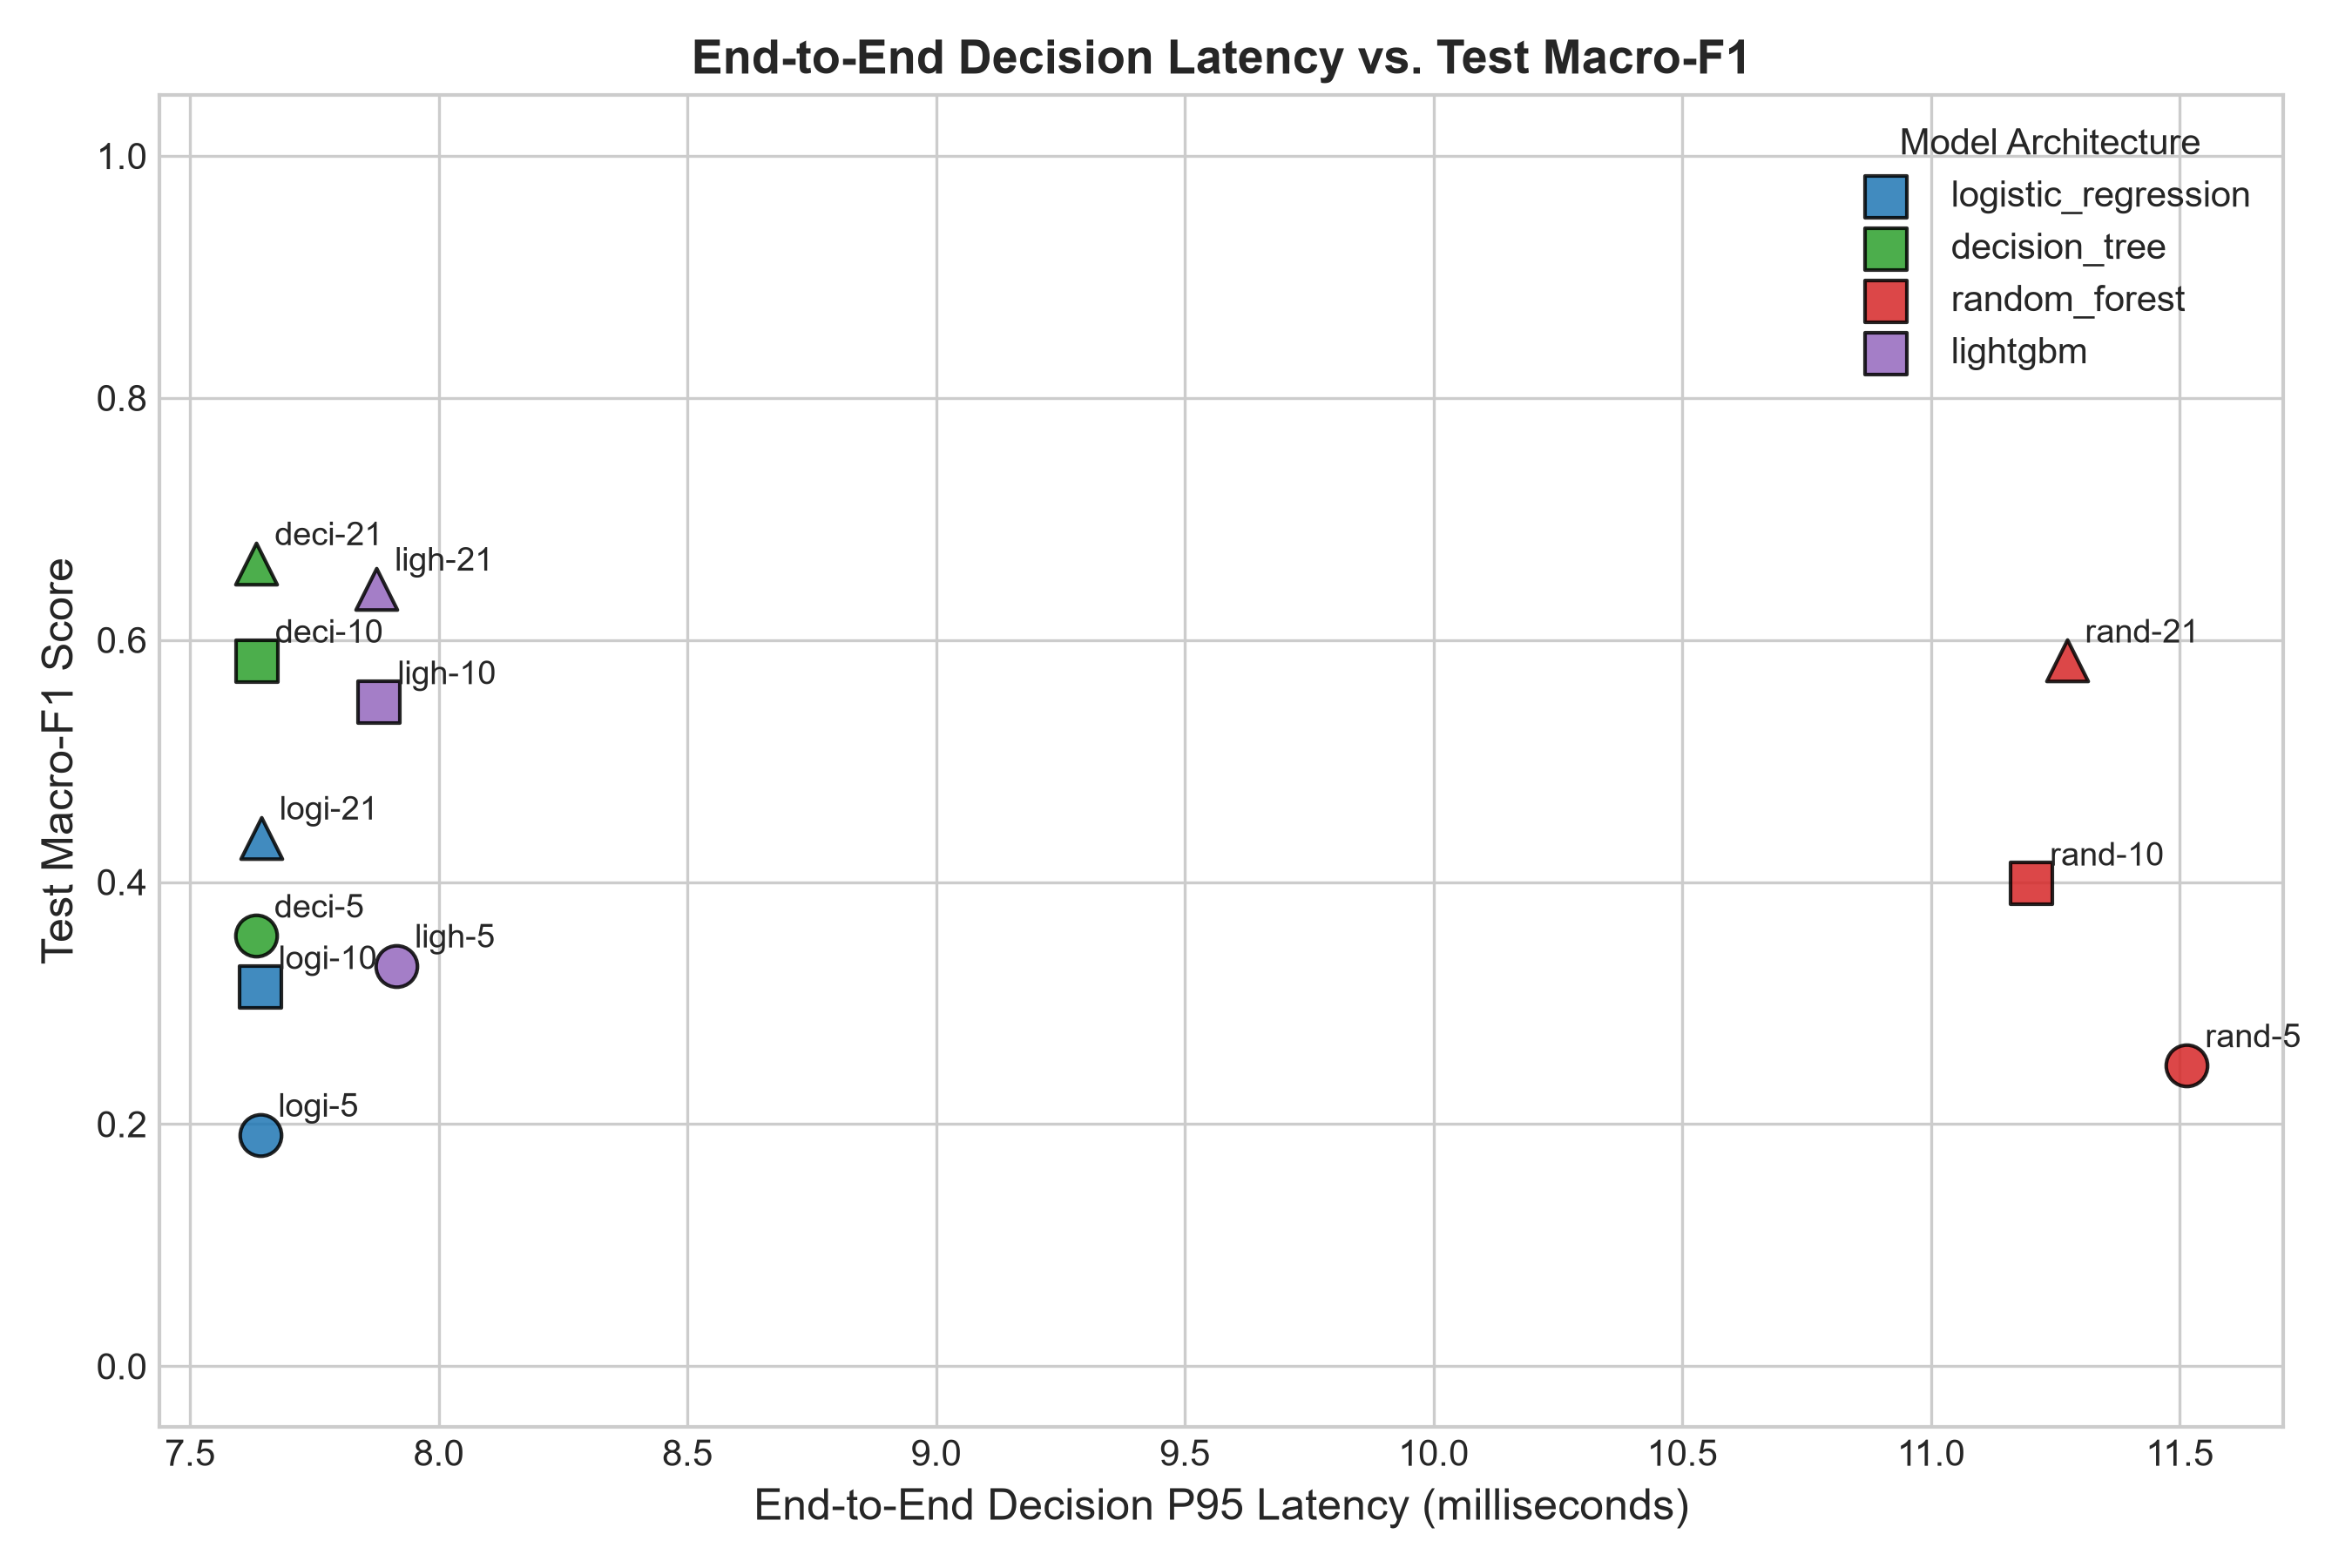
\includegraphics[width=0.95\columnwidth]{latency_vs_f1.png}
\caption{Macro-F1 vs. median inference latency Pareto frontier across architectures.}
\label{fig:latency_f1}
\end{figure}

Decision Tree vector inference executes in \textbf{0.0579~ms} ($57.9~\mu\text{s}$ P50, 15,600 flows/sec) with a \textbf{3.11~KB} serialized footprint and 289.60~MB RAM. Feature extraction requires 0.3856~ms P50, bounding total single-threaded pipeline throughput to 638.9 flows/sec. Live integration smoke tests (EXP-R15) sustained 81.78 predictions/sec across 142 packets and 15 flows with 0 dropped flows and zero payload persistence.

\section{Discussion}
\label{sec:discussion}

\subsection{Why Shallow Trees Match Ensembles}
In tabular network transport spaces, discriminative density is concentrated in a few orthogonal dimensions---primarily directionality asymmetry (\texttt{packet\_ratio}, \texttt{byte\_ratio}) and coarse volume (\texttt{total\_bytes}). Ensembling 100 trees provides an absolute gain of only +0.0071 Macro-F1 (+1.2\% relative) over a single Decision Tree, while imposing a $73\times$ latency penalty (4.25~ms vs. 0.058~ms) and a $56\times$ storage expansion (175.4~KB vs. 3.11~KB). When feature boundaries are approximately axis-aligned, bagging provides diminishing returns because error is governed by class overlap rather than variance.

\subsection{Mechanism of WireGuard Tunnel Degradation}
The transfer degradation from direct to WireGuard traffic ($\Delta\text{F1} = -0.2594$) is directly explained by protocol mechanics. Direct traffic exhibits multi-modal packet length distributions (e.g., small 60--120 byte TCP ACKs, 300--800 byte TLS ClientHello, and 1460-byte payload segments). WireGuard encapsulates all traffic within outer UDP packets, enforces a 1280-byte MTU, and adds 16-byte Poly1305 tags, compressing the length spectrum. Conversely, models trained on WireGuard traffic rely primarily on directionality ratios, which are preserved through encapsulation, enabling robust transfer to direct traffic (1.0000 Macro-F1).

\subsection{The Physical Delay Hierarchy}
Prior claims of ``microsecond real-time traffic classification'' commit a category error by reporting isolated CPU instruction timings. Physical packet arrival over real WAN connections requires tens to hundreds of milliseconds (64.04~ms for 3 packets, 331.38~ms for 5 packets). Wire delay constitutes $>80\%$ of operational classification time. Furthermore, waiting for retrospective full-flow termination takes $\approx 59.7$~seconds and fails (0.0000 Macro-F1) due to keep-alive packet dilution.

\section{Limitations and Threats to Validity}
\label{sec:limitations}

\subsection{Methodological and Algorithmic Limitations}
\begin{enumerate}
    \item \textbf{Closed-World 6-Class Assumption:} The supervised models assume a closed world over six canonical categories. While selective abstention ($\tau^* = 0.70$) filters ambiguous flows, the system is not an open-set anomaly detector. Unmodeled protocols with burst profiles resembling video streaming may produce false positives.
    \item \textbf{Multiplexed Protocol Overlap:} Modern applications blur traffic boundaries: dynamic Single Page Applications (SPAs) utilize WebSockets mimicking messaging, while enterprise platforms (Slack, Teams) multiplex text, voice, and video over identical QUIC connections. Disentangling multiplexed sub-flows using purely statistical features remains an open challenge.
    \item \textbf{Asymmetric Tunnel Transfer:} Classifiers trained on direct traffic cannot be deployed on VPN concentrators without explicit re-training on padded tunnel data.
\end{enumerate}

\subsection{Threat Model and Adversarial Evasion}
Zero-payload classifiers are vulnerable to active traffic morphing:
\begin{itemize}
    \item \textbf{Packet Padding:} Padding application payloads with random noise to 1460 bytes neutralizes packet length moments.
    \item \textbf{Timing Jitter Injection:} Injecting synthetic delays distorts inter-arrival time distributions.
    \item \textbf{Multipath Protocol Shuffling:} Distributing sessions across multipath QUIC fragments statistical signatures.
\end{itemize}
Our framework is intended for cooperative enterprise QoS and traffic monitoring, not defense against dedicated cryptographic obfuscators (e.g., Tor obfs4).

\subsection{Dataset Scale and Hardware Boundaries}
While \texttt{dataset\_v2} provides 301 flows and 150 independent sessions under strict group isolation, it represents an empirical hybrid benchmark on a single Windows 11 host. Pure physical Wi-Fi traffic without perturbations was evaluated on \texttt{dataset\_real\_v1} ($N=12$ test flows, 0.0833 Macro-F1). Multi-gigabit line-rate processing on $>10$~Gbps backbones requires re-implementing feature extraction in C/Rust using Linux eBPF/XDP kernel bypass.

\section{Conclusion and Future Work}
\label{sec:conclusion}

This paper presented an empirical evaluation of zero-payload encrypted traffic classification under strict group-aware session isolation. By disproving legacy claims of $>95\%$ Macro-F1 and demonstrating that Random Forest achieves 0.5854 Macro-F1 on a hybrid benchmark (and 0.0833 on pure physical Wi-Fi), we established the true empirical baseline of statistical metadata classification. We showed that a 3.11~KB Decision Tree achieves Pareto-optimal edge efficiency (0.5802 Macro-F1 in 0.0579~ms), directionality asymmetry carries the highest discriminative density, physical wire delay accounts for $>80\%$ of operational classification time, early triage at 3 packets achieves 0.6111 Macro-F1 in 79.94~ms, and validation-calibrated selective classification ($\tau^* = 0.70$) reduces decision error from 45.83\% down to 26.92\%. Future work will investigate multiplexed sub-flow disentanglement in QUIC and hardware-accelerated feature extraction via eBPF/XDP.

\section*{Acknowledgment}
The authors thank the Advanced Network Systems Laboratory for providing network testbed access and computing resources.

\bibliographystyle{IEEEtran}
\bibliography{references}

\end{document}
